\begin{abstract}
\Gls{md} simulations underpin modern computational drug discovery, materials science, and biochemistry. However, existing methods are notoriously expensive and time-consuming. In this light, we propose \gls{atoms}, a pretrained transformer neural operator for modeling 3D point cloud dynamics with a particular focus on predicting \gls{md} trajectories. \gls{atoms} shows excellent zero-shot generalization \textit{between} chemical compounds, demonstrating an average improvement of 44\% over leading equivariant graph approaches in multi-timestep atom-position \gls{mse}. To facilitate our own and future multitask operator learning, we introduce and publicly release TG80, the largest multi-compound \gls{md} benchmark dataset to date, comprising over 2.5 million femtoseconds of simulation data across 80 diverse compounds. Additionally, \gls{atoms} advances \gls{sota} performance on established single-task \gls{md} benchmarks, reducing \gls{mse} by 19\% on MD17 and 13\% on RMD17, surpassing prior best, EGNO. Our methodology capitalizes upon recent advancements in transformer pretraining (i.e., Muon, RoPE) and requires no prior knowledge of graph structure, unlike previous message-passing approaches. With \gls{atoms}, TG80, and the release of numerous pretrained checkpoints, we lay the groundwork for future research into \gls{md} neural operators with concrete scientific applicability.
\\
% \textbf{\gls{atoms} Code: \url{https://github.com/luke-a-thompson/gtno_py}} \\
% \textbf{\gls{atoms} Code: In supplementaries} \\
% \textbf{TG80 Dataset: In supplementaries}
\end{abstract} 

\section{Introduction}   
\glsresetall
Contemporary \gls{md} approaches leverage quantum-mechanical \gls{dft} simulations to calculate time series of atomic positions termed \textit{trajectories}. However, these methods scales extremely poorly with number of atoms $N$, with computational complexities ranging from \(\mathcal{O}(N^3)\) to \(\mathcal{O}(N^6)\) and requiring double-precision floating point computations, limiting GPU acceleration \cite{li_scaling_2024}.

Addressing this, recent works propose neural methods for tasks traditionally in the domain of \gls{dft} simulations. Neural \gls{md} architectures typically predict single-timestep forces and energies from a snapshot molecular conformation \cite{batatia_design_2022, batzner_e3-equivariant_2022, faber_alchemical_2018, gao_torchani_2020, gasteiger_gemnet_2021, kovacs_linear_2021, musaelian_learning_2022} or diffuse low-energy conformation states \cite{gu_aligning_2024,xu_geodiff_2022}. Current approaches to modeling per-atom positional dynamics are autoregressive, and as such, risk failing to capture multi-timestep temporal correlations or accumulating error as a function of trajectory length \cite{bengio_scheduled_2015, bergsma_sutranets_2023, taieb_bias_2016}. 

Furthermore, existing single-task models exhibit limited generalization to unseen chemical compounds, significantly restricting their scientific utility. Effective transfer learning in \gls{md} models is crucial for accurately predicting the dynamics of novel molecules, a necessity for advancing materials science and drug discovery.

In this light, we propose \gls{atoms}, a pretrained neural operator for molecular dynamics capable of zero-shot generalization to unseen chemical compounds, opening a new direction in operator learning with clear scientific applicability. Beyond \gls{atoms}, we:

\begin{enumerate}
    \item Release TG80, a \gls{md} dataset containing over 2.5 million femtoseconds of data across 80 compounds to serve as a robust benchmark for future multitask dynamics learning.
    \item Demonstrate \gls{sota} performance on our new dataset and the existing MD17 and RMD17 benchmarks, showing improvements of \(\%\) and \(\%\), respectively.
    \item Adapt \gls{nlp} approaches to operator learning, such as \gls{rope}, to encode temporal point cloud dynamics, and perform extensive ablations to evidence these changes and guide future neural operator research.
    \item Make numerous pretrained checkpoints available to establish a robust platform to support future research into efficient, scalable, and scientifically impactful neural operators for \gls{md}.
\end{enumerate}

\section{Related work}
\subsection{Equivariant Neural Networks}
Equivariance has emerged as an essential physics-informed prior for deep learning architectures operating on molecular data \cite{bronstein_geometric_2021, duval_hitchhikers_2023}. As a molecule's properties remain invariant under rotation, reflection, or other transformations, it follows that its latent representations should transform in a manner that preserves these symmetries. 

Early works in this domain employed convolutional approaches to achieve translation equivariance in E(3) \cite{weiler_3d_2018, wu_pointconv_2020} or tensor product attention and spherical harmonics to enforce roto-translational equivariance in SE(3) \cite{fuchs_se3-transformers_2020,thomas_tensor_2018}. In contrast, \gls{mpnn} frameworks, such as \gls{egnn} and others \cite{garcia_satorras_en_2021, gasteiger_gemnet_2021, huang_equivariant_2022}, achieve equivariance by operating on strictly equivariant features, such as inter-node distances and directions. While effective, \glspl{mpnn} typically presuppose a fixed molecular graph. This assumption is problematic as it fails to capture non-local interactions and dynamic bonding effects (e.g., resonances, transient interactions), which render predefined graphs inaccurate over time \cite{knutson_dynamic_2022,luo_predicting_2021}. Motivated by this, we instead model molecular trajectories as a series of point clouds, bypassing explicit graph construction and operating directly on the spatial configuration of atoms.

% Recent approaches have explored embeddings into geometric Clifford algebras to construct equivariant representations that capture higher-order multivector symmetries not preserved by traditional equivariant networks \cite{brehmer_geometric_2023, zhdanov_clifford-steerable_2024}. Orthogonal to these developments, \textcite{elhag_relaxed_2025} shows that non-equivariant architectures can be regularized to approximate equivariance with the addition of a loss term penalizing deviation from the expected transformation behavior under a given symmetry group.

\subsection{Neural operators}
Neural operators are deep learning architectures that learn discretization-invariant mappings between infinite-dimensional separable Banach spaces \cite{kovachki_neural_2021}. Xu et al. \cite{xu_equivariant_2024} bridge this framework and molecular dynamics by recasting the task as learning the solution operator of a differential equation that evolves past atomic positions into their future configurations.

A wide variety of neural architectures have been proposed for such operator learning. Notably, \gls{fno} \cite{li_fourier_2021} learns an operator in the Fourier domain, while its derivatives G-FNO \cite{helwig_group_2023} and PINO \cite{li_physics-informed_2023}, respectively, add group equivariance and physics-informed properties. \gls{egno} \cite{xu_equivariant_2024} intersperses \gls{egnn} and \gls{fno} layers to learn dynamic trajectories by capturing both spatial and temporal correlations.

Recently, transformer neural operators \cite{bryutkin_hamlet_2024,hao_gnot_2023,li_transformer_2023} have surpassed the performance of \gls{fno} in most \gls{pde} tasks. Notably, OFormer \cite{li_transformer_2023} uses a linear Galerkin-type attention mechanism, which omits the softmax and instead interprets the latent column vectors as basis functions. GNOT by \textcite{hao_gnot_2023} employs a novel subquadratic cross-attention methodology to integrate multiple feature types (e.g., shape and point relationships) into their transformer blocks. Another attentional approach is HAMLET \cite{bryutkin_hamlet_2024}, which constructs a graph of input observations and iteratively updates this representation using an encoder-decoder graph transformer. We unify the \gls{md} problem formulation and temporal discretization approach introduced by \gls{egno} with the increased representational power of transformers with \gls{atoms} by incorporating multi-feature spatio-temporal features into our attention computations.

\subsection{Existing MD Benchmarks}
Research into graph learning for molecular dynamics is marred by the \say{bad benchmarking culture,} which affects \gls{gnn} literature more broadly \cite{bechler-speicher_position_2025}. For example, despite MD17 benzene showing non-physical noise roughly 1000 times greater than that of other compounds, as reported by \textcite{christensen_revised_2020} in 2020, it is still regularly employed to benchmark new models \cite{bihani_egraffbench_2023,huang_equivariant_2022,liao_equiformer_2023, xu_equivariant_2024}. The practical relevance of single-task learning on these datasets is also dubious, as predicting trajectories for molecules with existing numerical solutions offers minimal benefit. We posit that the strengths of neural approaches emerge in transfer learning scenarios, where models generalize to unseen compounds, thereby circumventing the computational costs associated with explicit numerical simulations. This motivates our development of TG80 to facilitate multitask dynamics learning across molecular systems.

\section{Notations and Problem Formulation}
\subsection{Notations}
We consider a system state time \(t\) as a point cloud of \(N\) nodes, which we denote $\mathcal{G}^{(t)}$. Our objective is to predict a trajectory $\Delta t$ timesteps into the future, comprising a sequence of $P$ graphs $\{\mathcal{G}^{(t+\Delta t_p)}\}_{p=1}^{P}$ at increments $\Delta t_p$. For example, given an initial graph $\mathcal{G}^{(1000)}$ and choosing \(\Delta t = 3000, P=8\), we get the increments defined as $\Delta t_p = 3000 + (p-1)$ for $p = 1,\dots,8$. Thus, our aim is to estimate the sequence \(\{\mathcal{G}^{(4000)}, \mathcal{G}^{(4001)}, \dots, \mathcal{G}^{(4007)}\}\) using only the input state $\mathcal{G}^{(1000)}$.

\subsection{Problem Formulation}
We aim to learn a neural operator $F$, parameterized by $\theta$, approximating the ground-truth evolution operator $F^\dagger$. Given an input graph $\mathcal{G}^{(t)}$, the operator predicts a future trajectory by outputting states at discrete time increments \(\{ \Delta t_p \}\). The ideal learning objective is to minimize the expected squared $\ell_2$ distance between the predicted and actual future states over the trajectory horizon:
\begin{align}
    &\min_{\theta}\mathbb{E}_{\substack{
            \mathcal{G}^{(t)} \sim p_\text{data} \\
            }
        } \frac{1}{P} \sum_{p=1}^P
         \left\|
            F\left( \mathcal{G}^{(t)} ; \theta \right)(\Delta t_p) - F^\dagger \left (\mathcal{G}^{(t)} \right) (\Delta t_p)
        \right\|_{2}^{2}.
        \label{eq:objective_function}
\end{align}
Focusing on positional dynamics, we replace the true future state $F^\dagger(\mathcal{G}^{(t)})(\Delta t_p)$ with the known future ground truth node positions $\mathbf{x}'_{t+\Delta t_p}$. Introducing additive Gaussian noise $\xi \sim \mathcal{N}(0, \sigma^2)$ to the input features yields the practical objective function minimized in our work:
\begin{align}
    &\min_{\theta}\mathbb{E}_{\substack{
            \mathcal{G}^{(t)} \sim p_\text{data} \\
            \xi \sim \mathcal{N}(0, \sigma^2)
            }
        } \frac{1}{P} \sum_{p=1}^P
         \left\|
            F\left( \mathcal{G}^{(t)} + \xi ; \theta \right)(\Delta t_p) - \mathbf{x}^\dagger_{t+\Delta_{t_p}}
        \right\|_{2}^{2}.
        \label{eq:practical_objective_function}
\end{align}

\section{ATOM Architecture}
\begin{figure}[t]
    \centering
    \begin{subfigure}{0.72\linewidth}
        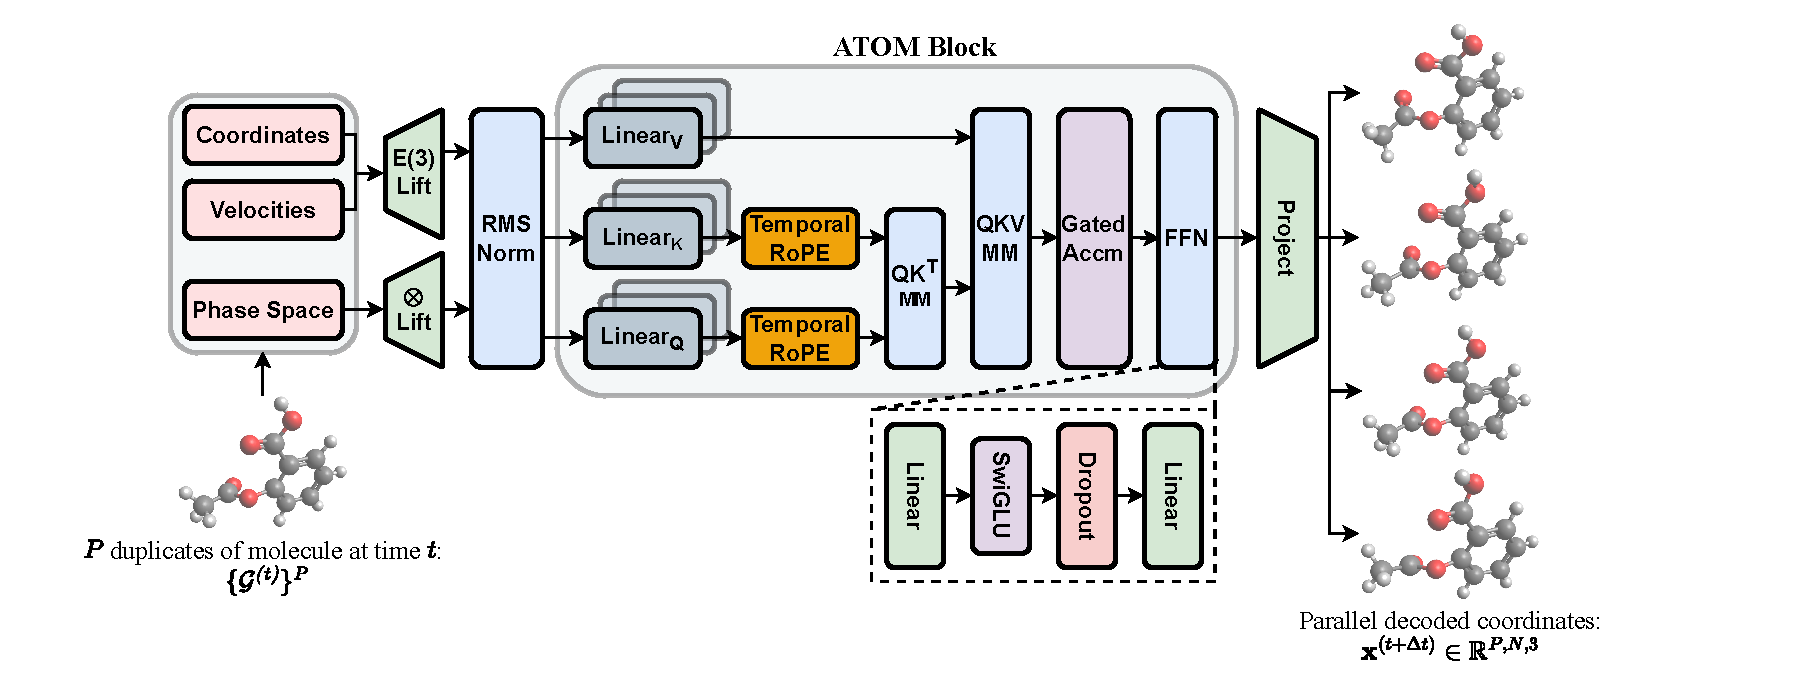
\includegraphics[trim=1cm 0cm 3.5cm 0cm, width=\linewidth]{Figures/GTNO_diagram-New RoPE.pdf}
        \caption{\gls{atoms}}
        \label{fig:atoms_arch}
    \end{subfigure}
    \hfill
    \begin{subfigure}{0.26\linewidth}
        \raisebox{0.4cm}{
            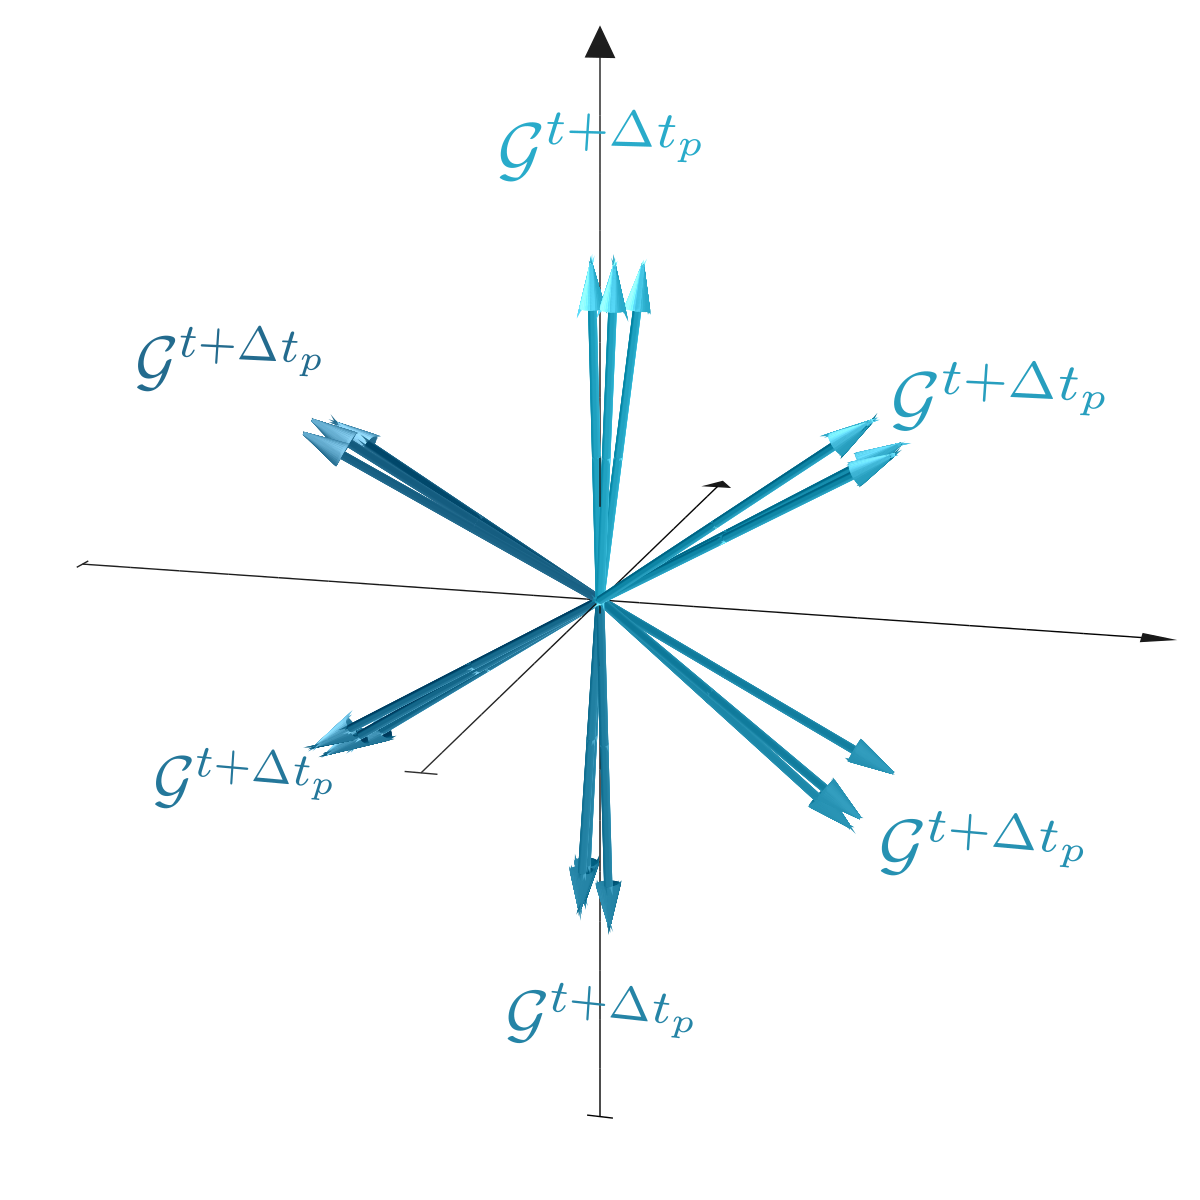
\includegraphics[width=\linewidth]{Figures/StaticTemporalRoPEVisualization_ManimCE_v0.19.0.png}
        }
        \caption{\gls{trope}}
        \label{fig:trope_arch}
    \end{subfigure}
    \caption{\gls{atoms} architecture. An input graph \(\mathcal{G}^{(t)}\) is repeated \(P\) times, yielding \(\{\mathcal{G}^{(t)}\}^{P}\). All node features are then equivariantly lifted to a unified embedding. Keys ($\mathbf{K}$) and values ($\mathbf{V}$) are generated for all features whilst we compute Queries ($\mathbf{Q}$) via a tensor product of the lifted phase space components. \gls{trope} progressively rotates each \(\mathcal{G}\) according to it's sequence position \(p\), as in \cref{fig:trope_arch}, and enriches \(\mathbf{Q}, \mathbf{K}\) with this temporal context. Features are finally summed and projected back to \(\mathbb{R}^3\) via a \(\mathrm{Project}\) \gls{mlp}, producing the decoded atom coordinates. During multitask training, we use a mixture-of-experts-like approach and learn several output heads with routing based on pooled molecular structure.}
    \label{fig:gnot-arch}
\end{figure}
\subsection{Learnable Noise}
\label{sec:learnable_noise}
Motivated by the beneficial regularization effect of label noise \cite{damian2021label,haochen2021shape}, we augment the ground-truth node  positions \(\mathbf{x}^\dagger_i\) and velocities \(\mathbf{v}^\dagger_i\) by independently sampling per-feature isotropic Gaussian noise \(\boldsymbol{\xi}_i \sim \mathcal{N}(\mathbf{0}, \sigma^2 \mathbf{I})\) each epoch:

\begin{equation}
    \mathbf{x}_i' = \mathbf{x}^\dagger_i + \boldsymbol{\xi}_\mathbf{x}, \qquad
    \mathbf{v}_i' = \mathbf{v}^\dagger_i + \boldsymbol{\xi}_\mathbf{v}.
\end{equation}

We only use the noisy ground truths during training and report all results on the actual ground truths. Similar approaches have been employed for \gls{md} \glspl{gnn} and neural operator pretraining \cite{dauparas_robust_2022, zhou2024strategies, hao2024dpot}. Random perturbations improve generalization by reducing overfitting to numerical artifacts; we observe that removing them markedly degrades performance, as shown in \cref{fig:MD17_ablation}.

\subsection{Equivariant Lifting}
\label{sec:equivariant_lifting}
Given 3-D atom positions and velocities augmented with their \(\ell_2\) norms,
\begin{equation}
    \mathbf{x} = (x,y,z,\sqrt{x^2+y^2+z^2}), \qquad \mathbf{v} = (v_x, v_y, v_z, \sqrt{v_x^2+v_y^2+v_z^2}) \in \mathbb{R}^4,
\end{equation}
we view each as carrying the irreducible representation \(V_{\text{in}} \coloneqq \rho^{\text{odd}}_1 \oplus \rho^{\text{even}}_0\) of \(E(3)\): an odd-parity vector and even-parity scalar channel. We then apply two \(E(3)\)-equivariant lifting layers with the lifting multiplicity hyperparameter \(m\) set to 32,
\begin{equation}
    f_{\mathbf{x}},f_{\mathbf{v}} \colon V_{\text{in}}\longrightarrow V \coloneqq \bigoplus_{k=1}^mV_{\text{in}}.
\end{equation}
The embedded features are then
\begin{equation}
    \tilde{\mathbf{x}} \coloneqq f_{\mathbf{x}}(\mathbf{x}),
    \qquad
    \tilde{\mathbf{v}} \coloneqq f_{\mathbf{v}}(\mathbf{v}),
\end{equation}
and \(V\) satisfies the equivariance constraints:
\begin{equation}
    f_{\mathbf{x}}(g\!\cdot\!\mathbf{x}) \;=\; \rho_V(g)\, \cdot f_{\mathbf{x}}(\mathbf{x}),
    \qquad
    f_{\mathbf{v}}(g\!\cdot\!\mathbf{v}) \;=\; \rho_V(g)\, \cdot f_{\mathbf{v}}(\mathbf{v}), 
    \quad 
    \forall g \in E(3).
\end{equation}
where $\cdot$ denotes the group action and $\rho_V(g)$ represents the group action of $g$ on $V$. 

To form each atom's phase space vector \(\mathbf{z}\), we first form the concatenation \(\hat{\mathbf{v}} = (\mathbf{v}||\mathcal{Z}) \in W_\text{in} := V_\text{in} \oplus \rho_0^\text{even}\), where the atomic number \(\mathcal{Z} \in \mathbb{N}_{>0}\) is an even-parity scalar. We pass this through another equivariant linear layer to form its lifted representation:
\begin{equation}
    f_{\hat{\mathbf{v}}} \colon W_\text{in} \to V,
    \qquad
    \tilde{\mathbf{v}}^* \coloneqq f_{\hat{\mathbf{v}}}(\hat{\mathbf{v}}).
\end{equation}
Finally, we form the phase space embedding using a fully-connected tensor product layer:
\begin{equation}
    \mathbf{z} = \sum_{k=1}^m W_k \Pi_k 
    [\tilde{\mathbf{x}} \otimes \tilde{\mathbf{v}}^*]
\end{equation}
where \(\Pi_k \colon V \otimes V \to V\) is the Clebsch-Gordan projector and \(W_k \in \mathbb{R}\) is a learnable matrix linearly mixing the projected irreps to yield \(\mathbf{z} \in V\). This construction enables the formation of a rich, symmetry-respecting phase space embedding that captures higher-order interactions between position, velocity, and mass features \cite{thomas_tensor_2018, fuchs_se3-transformers_2020}.

\subsection{Temporal RoPE}
\label{sec:trope}
\gls{rope} \cite{su_roformer_2023} is a positional embedding wherein latent query \(\textbf{Q}\) and key \(\textbf{K}\) representations are progressively rotated according to their position in the input sequence. In \gls{nlp} tasks, \gls{rope} consistently outperforms traditional sinusoidal positional encodings \cite{su_roformer_2023, barbero_round_2024}, which remain standard in neural operator architectures.

Motivated by this, we develop \gls{trope}, an adaptation of \gls{rope} for encoding the temporal order of point clouds in a dynamics trajectory. For a given timestep \(p\in\{1,\dots,P\}\) we define a single rotation angle
\(\theta_{p,k} = p \cdot \omega_k\) where the frequency spectrum \(\omega_k\) is scaled logarithmically as in \cite{su_roformer_2023}. Each hidden representation \(h_i\in\mathbb{R}^{d_{\text{head}}}\)
is split into \(\frac{d_{\text{head}}}{2}\) disjoint 2-D subspaces, and its own angle \(\theta_{p,k}\) is applied to each subspace, yielding:
\begin{equation}
    R_{p}\;=\;
    \operatorname{diag}\Bigl(R(\theta_{p,1}),\dots, R(\theta_{p,d_\text{head}/2})\Bigr)
    \;\in\;
    \mathbb{R}^{d_{\text{head}}\times d_{\text{head}}},
    \quad
    R(\theta)=
    \begin{bmatrix}
        \cos\theta & -\sin\theta\\[2pt]
        \sin\theta &  \cos\theta
    \end{bmatrix}.
    \label{eq:trope_single_angle}
\end{equation}
Repeating the same \(2\times2\) block preserves the phase-alignment property
proved for RoPE \cite{su_roformer_2023}, \(\langle R_pQ, R_pK \rangle = \langle Q, K \rangle\) as each block is orthogonal \(R_p^\top R_p = I\), ensuring temporal rotation
commutes with attention. We apply rotations in a manner \emph{equivalent} to the following Kronecker product:
\begin{equation}
    R = \begin{bmatrix}
    R_1\otimes I_N & \mathbf{0} & \cdots & \mathbf{0} \\[1mm]
    \mathbf{0} & R_2\otimes I_N & \cdots & \mathbf{0} \\[1mm]
    \vdots & \vdots & \ddots & \vdots \\[1mm]
    \mathbf{0} & \mathbf{0} & \cdots & R_P\otimes I_N
    \end{bmatrix} \in \mathbb{R}^{(PN \cdot d_{\text{head}}) \times (PN \cdot d_{\text{head}})},
\end{equation}
where \( I_N \) is the \( N \times N \) identity matrix. Thus, all points corresponding to the same timestep \(p\) have their hidden dimensions rotated identically to encode \(\mathcal{G}^{(t)} \in \{\mathcal{G}^{(t)}\}^P_{p=1}\). In practice, we use element-wise operations to avoid forming this large matrix, using only \(\mathcal{O}(PNd_\text{head})\) memory.
% \EScomment{Shall we use $\mathcal{G}^{(t)} \in \{\mathcal{G}^{(t)}\}^P_{t=1}$.}

The rotation angle for each timestep \( p \) is determined by scaling the integer time index with a set of frequencies. Specifically, we define the frequency vector as: 
\begin{equation}
    \boldsymbol{\omega} = \left(\frac{1}{\text{base}^{\frac{2i}{d_{\text{head}}}}} \right)_{i=0}^{\frac{d_{\text{head}}}{2} - 1}.
\end{equation}
Typical \gls{rope} bases are on the order of 10k to 1M for \gls{nlp} transformers \cite{su_roformer_2023, jiang_mixtral_2024, men_base_2024}. However, we hypothesized a \gls{trope} base of 1000 would beneficially exaggerate rotations to be more visible in our relatively small sequence lengths \(P = [8,16]\). Our experiments with varying bases studies did not provide conclusive evidence of any benefit (\cref{tab:trope_bases}).

\subsection{Cross-attention Block}
\label{sec:cross_attention}
Inspired by \cite{hao_gnot_2023}, we employ a cross-attention mechanism to enable mixing between different feature modalities. We first compute the queries \(\mathbf{Q}\) from the phase space \(\mathbf{z}\)
\begin{equation}
    \mathbf{Q} = \mathbf W_{Q}\mathbf{z} + \mathbf{b}_{Q}, 
\end{equation}
then the keys \(\mathbf{K}\) and values \(\mathbf{V}\) from the lifted positions and velocities:
\begin{equation}
     \quad \mathbf{K}^F =  \mathbf{W}_K F + \mathbf{b}_K, \quad \mathbf{V}^F =  \mathbf{W}_V F + \mathbf{b}_V, \qquad F \in \mathcal{F} = \{\tilde{\mathbf{x}}, \tilde{\mathbf{v}}\}.
\end{equation}

Considering the single-head case for simplicity, this yields the per-feature attention weights
\begin{equation}
    \mathbf{\alpha}^F = \operatorname{softmax} \Biggl( \frac{ \operatorname{T-RoPE}(\mathbf{Q}) \, \operatorname{T-RoPE}(\mathbf{K}^F)^\top}{\sqrt{d_h}} \Biggr),
\end{equation}
where \gls{trope} injects temporal positional information prior to softmax normalization and scaling. We then aggregate the feature-specific representation:
\begin{equation}
    \mathbf{A}^F = \alpha^F\mathbf{V}^F \label{eq:cross_attn}.
\end{equation}
To dynamically adjust the relative influence of different feature types, a gating mechanism learns scalar weight \( \gamma_F \in [0,1] \) per feature, then performs a softmax to weight each heterogeneous attention, \( \mathbf{A}^F \). An output transformation then combines these weighted features:
\begin{equation}
    \mathbf{x}_{\text{out}} = \mathbf{W}_O\Biggl( \sum_{F \in \mathcal{F}} \gamma_F \mathbf{A}^F \Biggr) + \mathbf{b}_O.
\end{equation}

Finally, we pass \(\mathbf{x}_{\text{out}}\) through an \gls{mlp}:
\begin{equation}
    \mathbf{x}_{\text{out}} = \operatorname{MLP}(\mathbf{x}_{\text{out}}).
\end{equation}

\begin{proposition}
\label{prop:kernel}
The cross-attention is equivalent to a kernel integral operator, i.e., ${\rm softmax}(\text{T-RoPE}(\mathbf Q) \text{T-RoPE}(\mathbf K^F)^\top/\sqrt{d_h}) \mathbf V^F = \int \kappa^F(\mathbf{z}, \mathbf{x}) v^F(x) d \mu_N(\mathbf{x})$, where $\kappa^F$ denotes the kernel induced by softmax function, $v^F(\mathbf x)$ denotes the values as a function of $\mathbf x$, and $\mu_N$ denotes the empirical measure supported on $\{ \mathbf{x}_i\}_{i=1}^N$. 
\end{proposition}


We remark that our kernel fails to satisfy global Lipschitz continuity \cite{delattre_efficient_2023}, unlike \gls{fno} \cite{li_fourier_2021}, and as such, certain generalization theorems fail \cite{le_mathematical_2024}.

\subsection{Projection}
\label{sec:project}
For the final output of \gls{atoms}, the predicted positions \(\mathbf{x}^\dagger\) are output via another \gls{mlp}, \(\operatorname{Project}\), which projects \(\mathbf{x}_\text{out}\) back to the target domain of \(3\)D space:
\begin{equation}
    \mathbf{x}^\dagger = \operatorname{Project}(\mathbf{x}_{\text{out}})
\end{equation}
In the multitask case, we employ an MoE-like approach detailed in \cref{sec:multi_head_output}.

\section{TG80 Dataset}
\begin{wrapfigure}{r}{0.4\linewidth}
  \vspace{-15pt}
  \centering
  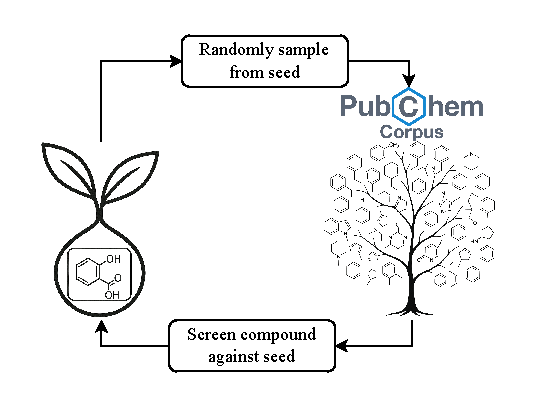
\includegraphics[width=\linewidth]{Figures/dataset/Dataset_diagram.pdf}
  \caption{Iterative construction of TG80 from an initial seed using the PubChem chemical database.}
  \label{fig:dataset_construction}
  \vspace{-15pt}
\end{wrapfigure}
We introduce TG80 as a superset of the MD17 dataset. Initially, our dataset comprises 40 seed molecules: the eight original MD17 compounds and 32 additional drug-like molecules selected through expert review. Over four iterations, we augment the seed dataset by selecting structurally similar molecules from the PubChem dataset of 173 million chemicals \cite{bolton_pubchem3d_2011}. Accepted candidates met Lipinski's criteria \cite{lipinski_experimental_2001} and showed 0.875–0.925 similarity to at least one seed compound by ECFP-4 fingerprint Tanimoto distance \cite{greg_landrum_rdkit_2012, rogers_extended-connectivity_2010,rogers_computer_1960}. We rejected molecules showing >0.80 similarity to those already selected from PubChem to prevent collapse to a highly similar data manifold.

We generate all \gls{md} trajectories using Orca V6.01 \cite{neese_software_2022} with the PBE functional \cite{perdew_generalized_1996}, DEF2-SVP \cite{weigend_balanced_2005, weigend_accurate_2006} basis set with \(\Delta\)4 dispersion corrections \cite{caldeweyher_generally_2019, caldeweyher_extension_2020, wittmann_extension_2024} at one femtosecond resolution in vacuum. This represents a common baseline methodology akin to RMD17, enhanced with more modern dispersion corrections to enhance stability and allow greater stepsize \cite{christensen_revised_2020}. As a result, we show generally superior numerical stability to both MD17 and RMD17 while covering a wider range of dynamics, as indicated by the variance of internal motion amongst compounds in TG80 \cref{fig:numerical_stability}. All simulations were performed using 32 AMD EPYC 7543 cores per molecule, consuming a total of 806 400 CPU hours with a quoted market cost of USD 150 000.

\section{Results}
We define two \gls{mse} metrics to evaluate \gls{atoms}. \textit{State-to-trajectory} (S2T) measures the average discrepancy between the predicted \(\mathbf{x}\) and ground-truth positions \(\mathbf{x}^\dagger\) across the entire sequence, while \textit{state-to-state} (S2S) quantifies the error at the final predicted timestep.
\begin{align}
    \operatorname{S2T} &= \frac{1}{P}\sum\limits_{p=1}^P\|\mathbf{x}_p - \mathbf{x}^\dagger_p\|_2^2, \\
    \operatorname{S2S} &= \|\mathbf{x}_P - \mathbf{x}^\dagger_P\|_2^2.
\end{align}
We report results using the lowest loss \(\operatorname{S2S}\) validation checkpoint and make all hyperparameters available in \cref{tab:gtno_hparams}. All results are in the form mean \(\pm 2\sigma\) gathered over three training runs.

\subsection{Single-task Learning on MD17, RMD17}
We assess performance on the MD17 and RMD17 datasets \cite{chmiela_machine_2017}, which each contain eight \gls{dft} \gls{md} trajectories. We partition the trajectories into train/validation/test splits of size 500/2000/2000, set \(\Delta t = 3000\), \(P = 8\) and train for 2 500 epochs.

\gls{atoms} achieves \gls{sota} results on MD17 aspirin, benzene, ethanol, salicylic acid, and toluene, substantially improving S2S and S2T test \gls{mse}. Specifically, our model reduces errors by \(61.58\%\) (S2S) and \(54.90\%\) (S2T) on benzene, and \(54.16\%\) (S2S) and \(50.66\%\) (S2T) on toluene, compared to the prior best (\gls{egno}). \gls{atoms} ranks second on malonaldehyde, naphthalene, and uracil, with the largest gap (\(8.90\%\)) in malonaldehyde, which we hypothesized to be due to implicit hydrogen representation inadequately modeling electron delocalization effects (see Appendix~\ref{tab:explicit_hydrogens}). In \cref{tab:rmd17_results} we show that \gls{atoms} also achieves leading results on the RMD17 dataset with a mean S2T improvement of 12\%, surpassing the previous \gls{sota} in all but one case.

% 2sigma
\begin{table}[ht]
    \centering
    \caption{MSE (\(\times 10^{-2}\)) on MD17. Upper part: S2S \gls{mse}. Lower part: S2T \gls{mse}.}
    \label{tab:md17_results}
    \resizebox{\linewidth}{!}{
    \begin{tabular}{lcccccccc}
        \toprule
        & Aspirin & Benzene & Ethanol & Malonaldehyde & Naphthalene & Salicylic & Toluene & Uracil \\
        \midrule
        RF \cite{kohler_equivariant_2019} & \(10.94{\scriptstyle \pm0.02}\) & \(103.72{\scriptstyle \pm2.58}\) & \(4.64{\scriptstyle \pm0.02}\) & \(13.93{\scriptstyle \pm0.06}\) & \(0.50{\scriptstyle \pm0.02}\) & \(1.23{\scriptstyle \pm0.04}\) & \(10.93{\scriptstyle \pm0.08}\) & \(0.64{\scriptstyle \pm0.02}\) \\
        TFN \cite{thomas_tensor_2018} & \(12.37{\scriptstyle \pm0.36}\) & \(58.48{\scriptstyle \pm3.96}\) & \(4.81{\scriptstyle \pm0.08}\) & \(13.62{\scriptstyle \pm0.16}\) & \(0.49{\scriptstyle \pm0.02}\) & \(1.03{\scriptstyle \pm0.04}\) & \(10.89{\scriptstyle \pm0.02}\) & \(0.84{\scriptstyle \pm0.04}\) \\
        SE(3)-Tr. \cite{fuchs_se3-transformers_2020} & \(11.12{\scriptstyle \pm0.12}\) & \(68.11{\scriptstyle \pm1.34}\) & \(4.74{\scriptstyle \pm0.02}\) & \(13.89{\scriptstyle \pm0.04}\) & \(0.52{\scriptstyle \pm0.02}\) & \(1.13{\scriptstyle \pm0.04}\) & \(10.88{\scriptstyle \pm0.12}\) & \(0.79{\scriptstyle \pm0.04}\) \\
        EGNN \cite{garcia_satorras_en_2021} & \(14.41{\scriptstyle \pm0.30}\) & \(62.40{\scriptstyle \pm1.06}\) & \(4.64{\scriptstyle \pm0.04}\) & \(13.64{\scriptstyle \pm0.02}\) & \(0.47{\scriptstyle \pm0.04}\) & \(1.02{\scriptstyle \pm0.04}\) & \(11.78{\scriptstyle \pm0.14}\) & \(0.64{\scriptstyle \pm0.02}\) \\
        EGNN-R \cite{garcia_satorras_en_2021} & \(14.51{\scriptstyle \pm0.38}\) & \(62.61{\scriptstyle \pm1.50}\) & \(4.94{\scriptstyle \pm0.08}\) & \(17.25{\scriptstyle \pm0.10}\) & \(0.82{\scriptstyle \pm0.04}\) & \(1.35{\scriptstyle \pm0.04}\) & \(11.59{\scriptstyle \pm0.08}\) & \(1.11{\scriptstyle \pm0.04}\) \\
        EGNN-S \cite{garcia_satorras_en_2021} & \(9.50{\scriptstyle \pm0.20}\) & \(66.45{\scriptstyle \pm1.78}\) & \(4.63{\scriptstyle \pm0.02}\) & \(12.88{\scriptstyle \pm0.02}\) & \(0.45{\scriptstyle \pm0.02}\) & \(1.00{\scriptstyle \pm0.04}\) & \(10.78{\scriptstyle \pm0.10}\) & \(0.60{\scriptstyle \pm0.02}\) \\
        EGNO \cite{xu_equivariant_2024} & \(9.18{\scriptstyle \pm0.12}\) & \(48.85{\scriptstyle \pm1.10}\) & \(4.62{\scriptstyle \pm0.02}\) & \(\textbf{12.80}{\scriptstyle \pm0.04}\) & \(\textbf{0.37}{\scriptstyle \pm0.02}\) & \(0.86{\scriptstyle \pm0.04}\) & \(10.21{\scriptstyle \pm0.10}\) & \(\textbf{0.52}{\scriptstyle \pm0.04}\) \\
        \gls{atoms} & \(\mathbf{6.52}{\scriptstyle \pm0.08}\) & \(\mathbf{18.78}{\scriptstyle \pm1.12}\) & \(\mathbf{3.47}{\scriptstyle \pm0.10}\) & \(13.51{\scriptstyle \pm0.10}\) & \(0.40{\scriptstyle \pm0.02}\) & \(\mathbf{0.83}{\scriptstyle \pm0.02}\) & \(\mathbf{4.68}{\scriptstyle \pm0.34}\) & \(0.55{\scriptstyle \pm0.02}\) \\
        \midrule
        \rowcolor{gray!20} Improvement (\%) & \(28.98\%\) & \(61.56\%\) & \(24.89\%\) & \(-5.55\%\) & \(-8.11\%\) & \(3.49\%\) & \(54.16\%\) & \(-5.77\%\) \\
        \midrule
    
        EGNN-R & \(12.07{\scriptstyle \pm0.22}\) & \(23.73{\scriptstyle \pm0.60}\) & \(3.44{\scriptstyle \pm0.34}\) & \(13.38{\scriptstyle \pm0.06}\) & \(0.63{\scriptstyle \pm0.02}\) & \(1.15{\scriptstyle \pm0.04}\) & \(5.04{\scriptstyle \pm0.04}\) & \(0.89{\scriptstyle \pm0.02}\) \\
        EGNN-S & \(9.49{\scriptstyle \pm0.24}\) & \(29.99{\scriptstyle \pm1.30}\) & \(3.29{\scriptstyle \pm0.02}\) & \(11.21{\scriptstyle \pm0.02}\) & \(0.43{\scriptstyle \pm0.02}\) & \(1.36{\scriptstyle \pm0.04}\) & \(4.85{\scriptstyle \pm0.08}\) & \(0.68{\scriptstyle \pm0.02}\) \\
        
    
        EGNO & \(7.37{\scriptstyle \pm0.14}\) & \(18.78{\scriptstyle \pm1.12}\) & \(3.28{\scriptstyle \pm0.04}\) & \(\mathbf{10.67}{\scriptstyle \pm0.02}\) & \(\mathbf{0.32}{\scriptstyle \pm0.02}\) & \(0.77{\scriptstyle \pm0.02}\) & \(4.58{\scriptstyle \pm0.06}\) & \(\mathbf{0.47}{\scriptstyle \pm0.02}\) \\
        \gls{atoms} & \(\mathbf{5.45}{\scriptstyle \pm0.28}\) & \(\mathbf{8.47}{\scriptstyle \pm0.50}\) & \(\mathbf{2.69}{\scriptstyle \pm0.10}\) & \(11.62{\scriptstyle \pm0.06}\) & \(0.37{\scriptstyle \pm0.02}\) & \(\textbf{0.71}{\scriptstyle \pm0.02}\) & \(\mathbf{2.26}{\scriptstyle \pm0.14}\) & \(0.54{\scriptstyle \pm0.02}\) \\
        \midrule
        \rowcolor{gray!20} Improvement (\%) & \(26.05\%\) & \(54.90\%\) & \(17.99\%\) & \(-8.90\%\) & \(-15.62\%\) & \(7.79\%\) & \(50.66\%\) & \(-14.89\%\) \\
        \bottomrule
    \end{tabular}
    }
\end{table}

\begin{figure}[H]
  \centering
  %---------- Left: Table ----------
  \begin{subfigure}{0.48\linewidth}
    \centering
    \caption{Big delta (\(\Delta t = 30\,000\)) S2S (upper) and S2T (lower) \gls{mse} (\(\times 10^{-2}\)) trajectory prediction on MD17.}
    \resizebox{\linewidth}{!}{%
      \begin{tabular}{lcccc}
        \toprule
         & Aspirin & Ethanol & Napthalene & Toluene \\
         \midrule
         \gls{egno} & \(31.63{\scriptstyle \pm0.12}\) & \(11.83{\scriptstyle \pm0.01}\) & \(1.19{\scriptstyle \pm0.00}\) & \(26.48{\scriptstyle \pm0.01}\) \\
         \gls{atoms} & \(\mathbf{7.03}{\scriptstyle \pm0.26}\) & \(\mathbf{4.97}{\scriptstyle \pm0.02}\) & \(\mathbf{0.54}{\scriptstyle \pm0.01}\) & \(\mathbf{21.98}{\scriptstyle \pm1.10}\) \\
         \midrule
         \gls{egno} & \(23.24{\scriptstyle \pm0.12}\) & \(9.13{\scriptstyle \pm0.00}\) & \(0.82{\scriptstyle \pm0.00}\) & \(24.90{\scriptstyle \pm0.03}\) \\
         \gls{atoms} & \(\mathbf{6.53}{\scriptstyle \pm0.12}\) & \(\mathbf{4.63}{\scriptstyle \pm0.05}\) & \(\mathbf{0.52}{\scriptstyle \pm0.00}\) & \(\mathbf{16.76}{\scriptstyle \pm0.68}\) \\
         \bottomrule
      \end{tabular}
    }
    \label{tab:big_delta_results}
  \end{subfigure}
  \hfill
  %---------- Right: Images ----------
  \begin{subfigure}{0.48\linewidth}
    \vspace{10pt}
    \centering
    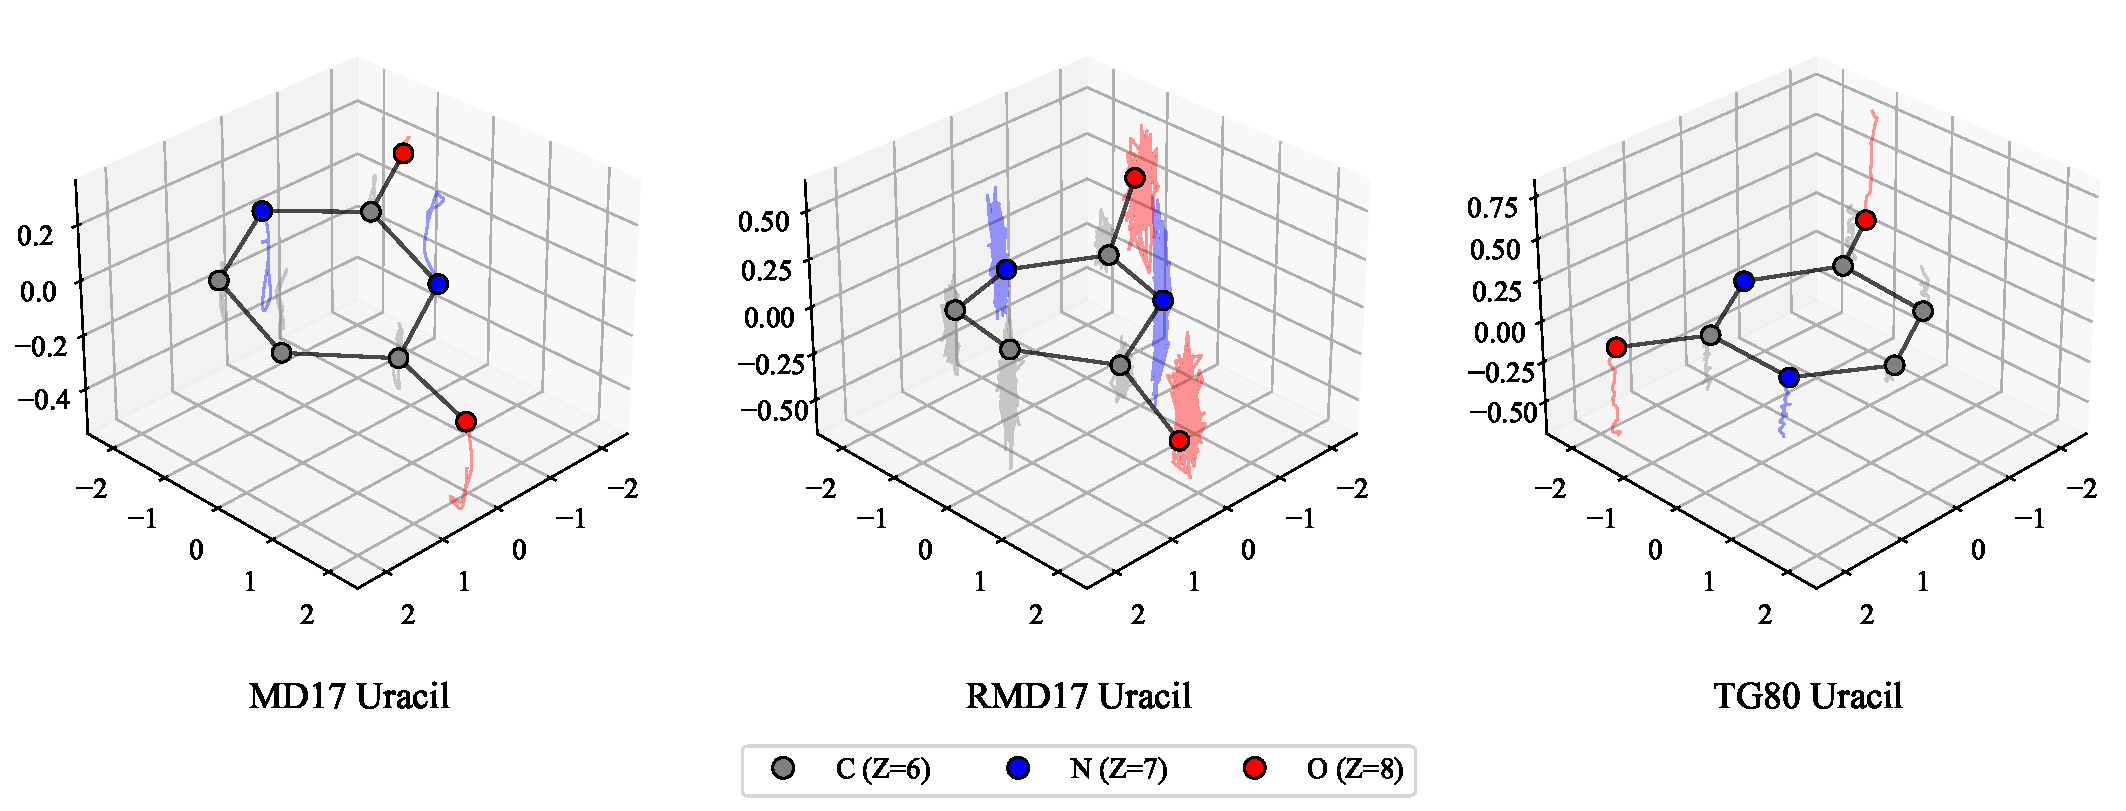
\includegraphics[width=\linewidth]{Figures/dataset/uracil_comparison.pdf}
    \caption{3000 timepoints of Uracil trajectory.}
    \label{fig:aspirin}
  \end{subfigure}
\end{figure}

\paragraph{Large \(\Delta t\) MD17}
Large time-horizon (\(\Delta t\)) \gls{md} simulations necessitate high-precision methods to prevent the accumulation of integration error over time \cite{liang_energy_2023}. As shown in \cref{tab:big_delta_results}, \gls{atoms} significantly outperforms \gls{egno}~\cite{xu_equivariant_2024} for large \(\Delta t\) prediction across four molecules in MD17, reducing S2S MSE by \(77.8\%\) for aspirin and \(58.1\%\) for toluene. Similar trends hold for S2T \gls{mse}.

\subsection{Multitask Learning on TG80}
We assess \gls{atoms}' zero‐shot generalisation on TG80. We train for 1\,000 epochs over five runs, randomly splitting molecules into training (6\,500), validation (13\,000) and test (13\,000) sets with a challenging $\Delta t = 10\, 000\,$fs. This exposes models to a broader range of dynamical behaviours than MD17.

In the multitask (MT) setting, \gls{atoms} MT halves the S2T \gls{mse} of \gls{egno} MT, with an average improvement of $43.7\%$ across five folds \cref{tab:tg80_single_task}. \gls{atoms} ZS outperforms specialised single‐task (ST) models across all evaluated molecules, despite no target‐specific training, achieving up to $26.4\%$ lower S2T \gls{mse} on Nitrobenzene and $20.1\%$ on Indole. This striking zero‐shot generalisation, realised without any exposure to the test molecules, confirms that multitask training endows \gls{atoms} with robust, transferable knowledge of molecular dynamics that single‐task models cannot match.

\begin{table}[H]
    \centering
    \begin{minipage}{0.48\linewidth}
        \caption{Multitask S2T \gls{mse} \(\pm2\sigma\) on TG80 across two runs per fold.}
        \resizebox{\linewidth}{!}{
        \begin{tabular}{lccccc}
            \toprule
            & Fold 1 & Fold 2 & Fold 3 & Fold 4 & Fold 5 \\
            \midrule
            \gls{egno} MT & \(187.10 \pm 27.61\) & \(179.14\pm10.36\) & \(165.77 \pm 9.82\) & \(201.73 \pm 10.88\) & \(195.42 \pm 10.00\) \\
            \gls{atoms} MT & \(93.74 \pm 0.84\) & \(91.27 \pm 0.85\) & \(85.17 \pm 2.47\) & \(105.97 \pm 1.27\) & \(149.28 \pm 5.67\) \\
            \midrule
            \rowcolor{gray!20} Improvement (\%) & 49.83\% & 49.05\% & 48.62\% & 47.47\% & 23.61\% \\
            \bottomrule
        \end{tabular}
        }
    \end{minipage}
    \hfill
    \begin{minipage}{0.48\linewidth}
        \caption{Single-task S2T \gls{mse} \(\pm 2\sigma\) on TG80 with three runs per fold.}
        \resizebox{\linewidth}{!}{
        \begin{tabular}{lccccc}
            \toprule
            & Uracil & Nitrobenzene & Indole & Naphtalene & Butanol \\
            \midrule
            \gls{egno} ST & \(233.92{\scriptstyle \pm10.56}\) & \(288.37{\scriptstyle \pm12.70}\) & \(232.48{\scriptstyle \pm10.23}\) & \(250.44{\scriptstyle \pm11.72}\) & \(182.04{\scriptstyle \pm8.74}\) \\
            \gls{atoms} ZS & \(93.34\) & \(91.28\) & \(83.96\) & \(105.32\) & \(109.92\) \\
            \gls{atoms} ST & \(97.84{\scriptstyle \pm2.16}\) & \(124.06{\scriptstyle \pm4.94}\) & \(105.08{\scriptstyle \pm1.55}\) & \(123.26{\scriptstyle \pm4.10}\) & \(85.49{\scriptstyle \pm1.33}\) \\
            \midrule
            \rowcolor{gray!20} Improvement (\%) \\
            \bottomrule
        \end{tabular}
        }
    \end{minipage}
    \label{tab:tg80_single_task}
\end{table}

\subsection{\(P, \Delta t\) Invariance Properties}
We evaluate the robustness of \gls{atoms} and \gls{egno} with respect to discretization granularity and the temporal gap \(\Delta t\). We fix \(P=8\) and vary \(\Delta t\) logarithmically from \(300\) to \(100\ 000\). As seen in \cref{fig:delta_t_invariance}, \gls{atoms} maintains near-constant S2T \gls{mse} across the range whilst the current \gls{sota}, \gls{egno}, exhibits deteriorating performance as \(\Delta t\) increases. This \(\Delta t\) invariance is practically desirable as long trajectories are expensive to numerically integrate with current DFT approaches and allow simulation of rare dynamical events \cite{piccini_ab_2022, li_scaling_2024}.

Both \gls{atoms} and \gls{egno} show consistent S2T \gls{mse} as \(P\) is varied from \(4\) to \(16\) in \cref{fig:p_invariance}. Such behaviour is expected following the discretization invariance property of neural operators \cite{kovachki_neural_2021}.

\begin{figure}[H]
    \centering
    \begin{subfigure}{0.48\linewidth}
        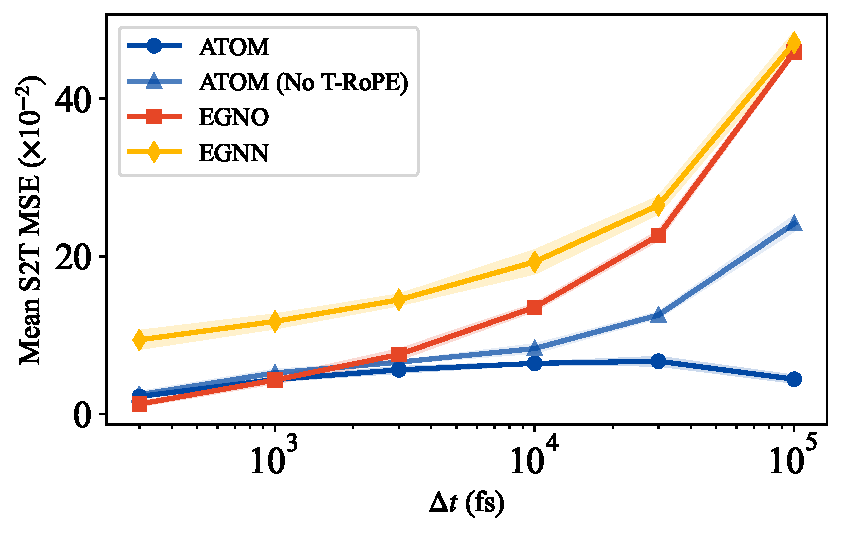
\includegraphics[width=\linewidth]{Figures/invariances/t_invariance_results.pdf}
        \caption{S2T \gls{mse} across \(\Delta t\). \gls{atoms} maintains near-constant error as \(\Delta t\) is varied, as opposed to previous approaches, which show diminishing performance.}
        \label{fig:delta_t_invariance}
    \end{subfigure}
    \hfill
    \begin{subfigure}{0.48\linewidth}
        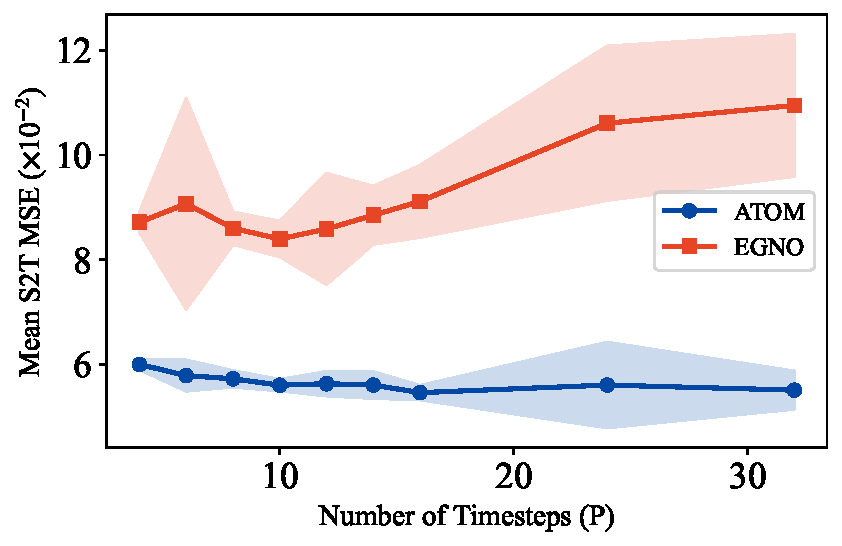
\includegraphics[width=\linewidth]{Figures/invariances/p_invariance_results.pdf}
        \caption{S2T \gls{mse} across \(P\). \gls{atoms} and \gls{egno} both maintain consistent loss across the range of \(P\) following discretization invariance.}
        \label{fig:p_invariance}
    \end{subfigure}
    \label{fig:invariances}
\end{figure}

\subsection{Ablations}
We perform extensive ablations on MD17 to verify the benefits of our architectural developments.

\paragraph{Input Noise}
\FPeval{\NoNoisevsDefault}{round(8.13 - 6.92, 2)}
Supporting our claim in \cref{sec:learnable_noise}, removing Gaussian noise from the input features increased S2T \gls{mse} by \NoNoisevsDefault{} on MD17.

\FPeval{\NoEquivariantLiftingvsDefault}{round(29.40 - 6.92, 2)}
\paragraph{Equivariant Lifting} We find that replacing the equivariant lifting introduced in \cref{sec:equivariant_lifting} with standard linear layers destroys the learning capacity of \gls{atoms}, increasing S2T \gls{mse} by \NoEquivariantLiftingvsDefault{}. This observation underscores the fundamental necessity of equivariance for modelling three-dimensional positional dynamics.

\paragraph{Cross-attention} To verify the importance of our cross-feature attention introduced in \cref{sec:cross_attention}, we train \gls{atoms} with standard multi-head self-attention on the phase space \(\mathbf{z}\) alone and find it moderately degrades performance.

% No-TROPE - Default
\FPeval{\CrossAttNoPEvsDefault}{round(7.64 - 6.92, 2)}
\FPeval{\StdAttNoPEvsDefault}{round(7.91 - 7.39, 2)}
\paragraph{\gls{trope}} 
Ablating \gls{trope} hindered the performance of cross-attention and self-attention \gls{atoms} models, suggesting \gls{nope} schemes may be unsuitable for training transformer neural operators \cite{kazemnejad_impact_2023}. 
Interestingly, removing \gls{trope} from our cross-attention produces a degradation of \CrossAttNoPEvsDefault{}, larger than the degradation of \StdAttNoPEvsDefault{} when removing \gls{trope} from standard attention. We hypothesize that this prevents the learning of effective, temporally linked cross-modal representations. Finally, in \cref{tab:trope_bases}, we show that smaller \gls{rope} bases have little effect on model performance.

\paragraph{Further Architectural Elements}
Following \cite{garcia_satorras_en_2021}, we implemented a delta update as described in \cref{sec:delta_prediction}, finding no performance benefit over our MD17 baseline. Inspired by promising results on NanoGPT speedrunning \cite{jordan_nanogpt_2024}, we found learnable value residuals (\cref{sec:value_residuals}) \cite{zhou_value_2024} have a minor positive effect on \gls{mse}. 

\begin{figure}[H]
\centering
\begin{minipage}[t]{0.60\linewidth}
    \centering
    \includegraphics[width=\linewidth]{Figures/ablation_MD17.pdf}
    \caption{\gls{atoms} ablation on MD17 Aspirin.}
    \label{fig:MD17_ablation}
\end{minipage}
\hfill
\begin{minipage}[t]{0.38\linewidth}
    \centering
    \vspace{-130pt}
    \captionof{table}{S2T \gls{mse} across varying \gls{trope} bases and \(P\).}
    \label{tab:trope_bases}
    \resizebox{\linewidth}{!}{
    \begin{tabular}{lcc}
        \toprule
        Base & \(P=8\) & \(P=16\) \\
        \midrule
        100 & \(5.41{\scriptstyle \pm0.13}\) & \(5.41{\scriptstyle \pm0.13}\) \\
        1000 & \(5.61{\scriptstyle \pm0.04}\) & \(5.38{\scriptstyle \pm0.31}\) \\
        10\,000 & \(5.57{\scriptstyle \pm0.04}\) & \(5.39{\scriptstyle \pm0.05}\) \\
        100\,000 & \(5.69{\scriptstyle \pm0.13}\) & \(5.52{\scriptstyle \pm0.26}\) \\
        \bottomrule
    \end{tabular}
    }
\end{minipage}
\end{figure}

\section{Discussion}
\paragraph{Limitations} TG80 does not contain \gls{dft} trajectories for large polycyclic molecules with more than 15 heavy atoms, despite their obvious chemical and pharmacological relevance. In follow-on work, we intend to enrich TG80 with such molecules, calculated with a higher resolution DFT basis set, \(\omega\)B97X-3c \cite{muller_omegab97x-3c_2023}.

With \gls{atoms}, we demonstrate that carefully designed transformer neural operators enable zero-shot generalization to unseen chemical dynamics. Our experiments on existing and new datasets show that well-founded \gls{nlp} approaches can achieve \gls{sota} performance in \gls{md}, even without explicit graph representations. In combination with our TG80 dataset, we provide a large-scale open-source benchmark to evaluate future models and spur further operator research with concrete scientific applicability.

\newpage

\printbibliography

\appendix
% \section{Background}
% \subsection{Groups}
% A group \( (G, \circ) \) consists of a non-empty set \( G \) and a binary operation \(\circ: G \times G \to G\) satisfying the following axioms:
% \begin{enumerate}
%     \item \textbf{Closure:} For all \( a, b \in G \), the result of the operation \( a \circ b \) is also in \( G \): \( a \circ b \in G \).
%     \item \textbf{Identity Element:} There exists an element \( e \in G \) such that, for all \( a \in G \), \( a \circ e = e \circ a = a \).
%     \item \textbf{Associativity:} For all \( a, b, c \in G \), \( (a \circ b) \circ c = a \circ (b \circ c) \).
%     \item \textbf{Inverses:} For each \( a \in G \), there exists an element \( a^{-1} \in G \) such that \( a \circ a^{-1} = a^{-1} \circ a = e \).
% \end{enumerate}

% In general, not all groups are abelian. That is, the binary operation \(\circ\) does not necessarily commute:  
% \[
% g \circ h = h \circ g, \quad \forall g,h \in G.
% \]

% \subsection{Group Representations}
% A group representation is a homomorphism  \(\rho: G \to GL(V)\) that assigns an \(n \times n\) matrix to each group element \(g \in G\), realizing it as a linear transformation. Representations must preserve the binary operation for all members of the group \(G\) such that:
% \[
% \rho(g \circ h) = \rho(g) \rho (h), \quad \forall g,h \in G.
% \]

% A representation is reducible if it can be represented as the direct sum of other representations:
% \[
% \rho(g) = \rho_1(g) \oplus \rho_2(g), \quad \forall g \in G.
% \]

% For example, a reducible \(4 \times 4\) representation of \(SU(2)\) can be decomposed into two \(2 \times 2\) subrepresentations:

% \[
% \rho(g) =
% \begin{bmatrix}
% \rho_1(g) & 0 \\
% 0 & \rho_2(g)
% \end{bmatrix}, \quad \forall g \in SU(2),
% \]

% where \(\rho_1(g)\) and \(\rho_2(g)\) are the following irreducible representations of \(SU(2)\):

% \[
% \rho_1(g) =
% \begin{bmatrix}
% e^{i\theta} & 0 \\
% 0 & e^{-i\theta}
% \end{bmatrix}, \quad
% \rho_2(g) =
% \begin{bmatrix}
% e^{i\phi} & 0 \\
% 0 & e^{-i\phi}
% \end{bmatrix}.
% \]
% By contrast, irreducible representations or \textit{irreps} cannot be represented as a direct sum. Formally, they have no non-trivial invariant subspaces \(W \subset V\) such that:
% \[
% \rho(g)W \subset W, \quad \forall g \in G.
% \]
% Representing inputs as irreps ensures equivariance by constraining each feature to transform predictably under group actions. Given \( V = \bigoplus_{i} V_i \) with irreps \( V_i \), the transformation of an input \( x \in V \) under \( g \in G \) is:  
% \[
% \rho(g)x = \bigoplus_{i} \rho_i(g)x_i.
% \]  
% Each component \( x_i \) transforms independently according to \(\rho_i\), preserving symmetry. Scalars remain invariant, while vectors rotate according to standard representations. This decomposition prevents the mixing of differently transforming features, ensuring that all subsequent operations, linear or non-linear, respect the group’s symmetry, thereby maintaining equivariance throughout the network.

% \subsection{Tensor Products}
% \label{sec:tensor_products}
% Schur's lemma implies that there are no non-trivial linear equivariant maps that mix features decomposed into irreps. Specifically, for irreps \(\rho_i\) and \(\rho_j\), any linear map \(T: V_i \to V_j\) satisfying  
% \[
% T \rho_i(g) = \rho_j(g) T, \quad \forall g \in G,
% \]
% is either the zero map or an isomorphism if \(\rho_i \not\cong \rho_j\). Consequently, direct linear mixing between features transforming under distinct irreps is prohibited.

% Tensor products are employed to enable equivariant mixing. Given features \(x_i \in V_i\) and \(x_j \in V_j\), their tensor product \(x_i \otimes x_j\) transforms as 
% \[
% x_i \otimes x_j \mapsto (\rho_i \otimes \rho_j)(g)(x_i \otimes x_j) = \rho_i(g) x_i \otimes \rho_j(g) x_j,
% \]
% where \((\rho_i \otimes \rho_j)(g) = \rho_i(g) \otimes \rho_j(g)\). The resulting reducible representation decomposes into a direct sum of irreps:
% \[
% V_i \otimes V_j \cong \bigoplus_{k} V_k.
% \]
% This decomposition introduces new irreps \(V_k\) that permit non-trivial equivariant interactions. By projecting onto these irreps, networks can achieve feature mixing while preserving symmetry constraints.

% \subsection{Spherical Harmonics}
% Analogous to the Fourier series on the unit sphere, spherical harmonics \(Y_j\) form an orthonormal basis for the Hilbert space of square-integrable functions defined on the sphere \(L^2(S^2)\). Any function \(f(x) \in L^2(S^2)\) can be expressed in terms as:
% \begin{equation}
%     f(x) = \sum_{J \geq 0} \mathbf{f}_{J}^{\top}Y_{J},
% \end{equation}
% where the vector of coefficients \(f_J\) can be obtained via:
% \begin{equation}
%     \mathbf{f}_J = \int_{S^2}f(x)Y_{J}^*(x)dx.
% \end{equation}

% The spherical harmonics exhibit a predictable transformation property under rotations. For a rotation \(g \in G\), represented by the operator \(R_g\) on the sphere, they transform as:
% \begin{equation}
%     Y_J(R_g^{-1}x) = D_J^*(g) Y_J(x),
% \end{equation}
% where \(x \in S^2\). Here, \(D_J^*(g)\) is the complex conjugate of the \(J\)-th Wigner-D matrix, which acts on the \((2J+1)\)-dimensional space of harmonics of degree \(J\).

\section{Datasets}
\label{sec:dataset_construction}
\subsection{Model Inputs and the Dataloader}
We broadly follow \cite{shi_learning_2021, xu_equivariant_2024} in our dataset construction. We model hydrogen atoms implicitly and concatenate the position and velocity norms for each node \(i\) with their respective vectors. Unlike their implementations, we avoid explicit graph construction and do not include edge labels describing atomic bond types.

We reimplement the MD17 dataloader with a focus on improved throughput. Unlike previous versions~\cite{huang_equivariant_2022, xu_equivariant_2024}, which duplicate each input frame \(\mathcal{G}^{(t)} \to \{\mathcal{G}^{(t)}\}^{P}\) during every forward pass, our implementation performs this duplication and graph construction (if desired) during initialization. These modifications improve dataloader throughput by \(>5 \times\). The code is available at: \textbf{Anonymized  for review}
% \url{https://github.com/luke-a-thompson/gtno_py/blob/main/src/gtno_py/dataloaders/egno_dataloder.py}

\begin{table}[ht]
    \centering
    \caption{Mean time (seconds) to produce \(10\ 000\) batches over \(100\) benchmark runs. Batch size \(= 100\), \(500\) samples, \(\Delta t = 3000\). We allow \(500\) warmup batches and report \(2\sigma\) confidence intervals.}
    \label{tab:dataloader_perf}
    \begin{tabular}{lcccc}
        \toprule
         & Aspirin & Ethanol & Naphthalene & Toluene \\
         \midrule
         \gls{egno} & \(0.060{\scriptstyle \pm0.024}\) & \(0.024{\scriptstyle \pm0.016}\) & \(0.056{\scriptstyle \pm0.024}\) & \(0.039{\scriptstyle \pm0.024}\) \\
         \gls{atoms} & \(0.005{\scriptstyle \pm0.002}\) & \(0.007{\scriptstyle \pm0.002}\) & \(0.008{\scriptstyle \pm0.004}\) & \(0.006{\scriptstyle \pm0.002}\) \\
         \bottomrule
    \end{tabular}
\end{table}

\subsection{Dataset Generation Algorithm}
We compute TG80 with the same PBE functional used for MD17 and RMD17, augmenting it with state-of-the-art \(\Delta 4\) dispersion corrections; as \cref{fig:numerical_stability} illustrates, this contributes to superior numerical stability.

\subsection{DFT Theory}
\begin{table}[H]
    \centering
    \caption{An overview of the functions, dispersion correction techniques, and basis sets used in \gls{md} datasets featured.}
    \label{tab:dft_techniques}
    \begin{tabular}{lcccc}
        \toprule
        & \gls{dft} Functional & Dispersion Corrections & Basis set & Timestep \\
        \midrule
        MD17 \cite{chmiela_machine_2017} & PBE & TS & NAO & \(0.5\) fs \\
        RMD17 \cite{christensen_role_2020} & PBE & N/A & def2-SVP & \(0.5\) fs \\
        TG80 & PBE & \(\Delta 4\) & def2-SVP & \(1.0\) fs \\
        \bottomrule
    \end{tabular}
\end{table}

We evaluate the numerical stability of MD17, RMD17 and TG80. MD17 benzene clearly shows substantial centre of mass drift in \cref{fig:MD17_numerical_quality}, which is also partially visible by the consistent motion trails shown in \cref{fig:MD17_trajectories}. RMD17 shows much improved stability, with centre of mass drift not exceeding \(10^4\). TG80 shows the lowest drift of all datasets examined, and expectedly includes more molecules with high per-step drift (due to more complex sterically hindered geometries).
\subsection{Numerical stability}
\begin{figure}[H]
    \begin{subfigure}{0.48\textwidth}
        \centering
        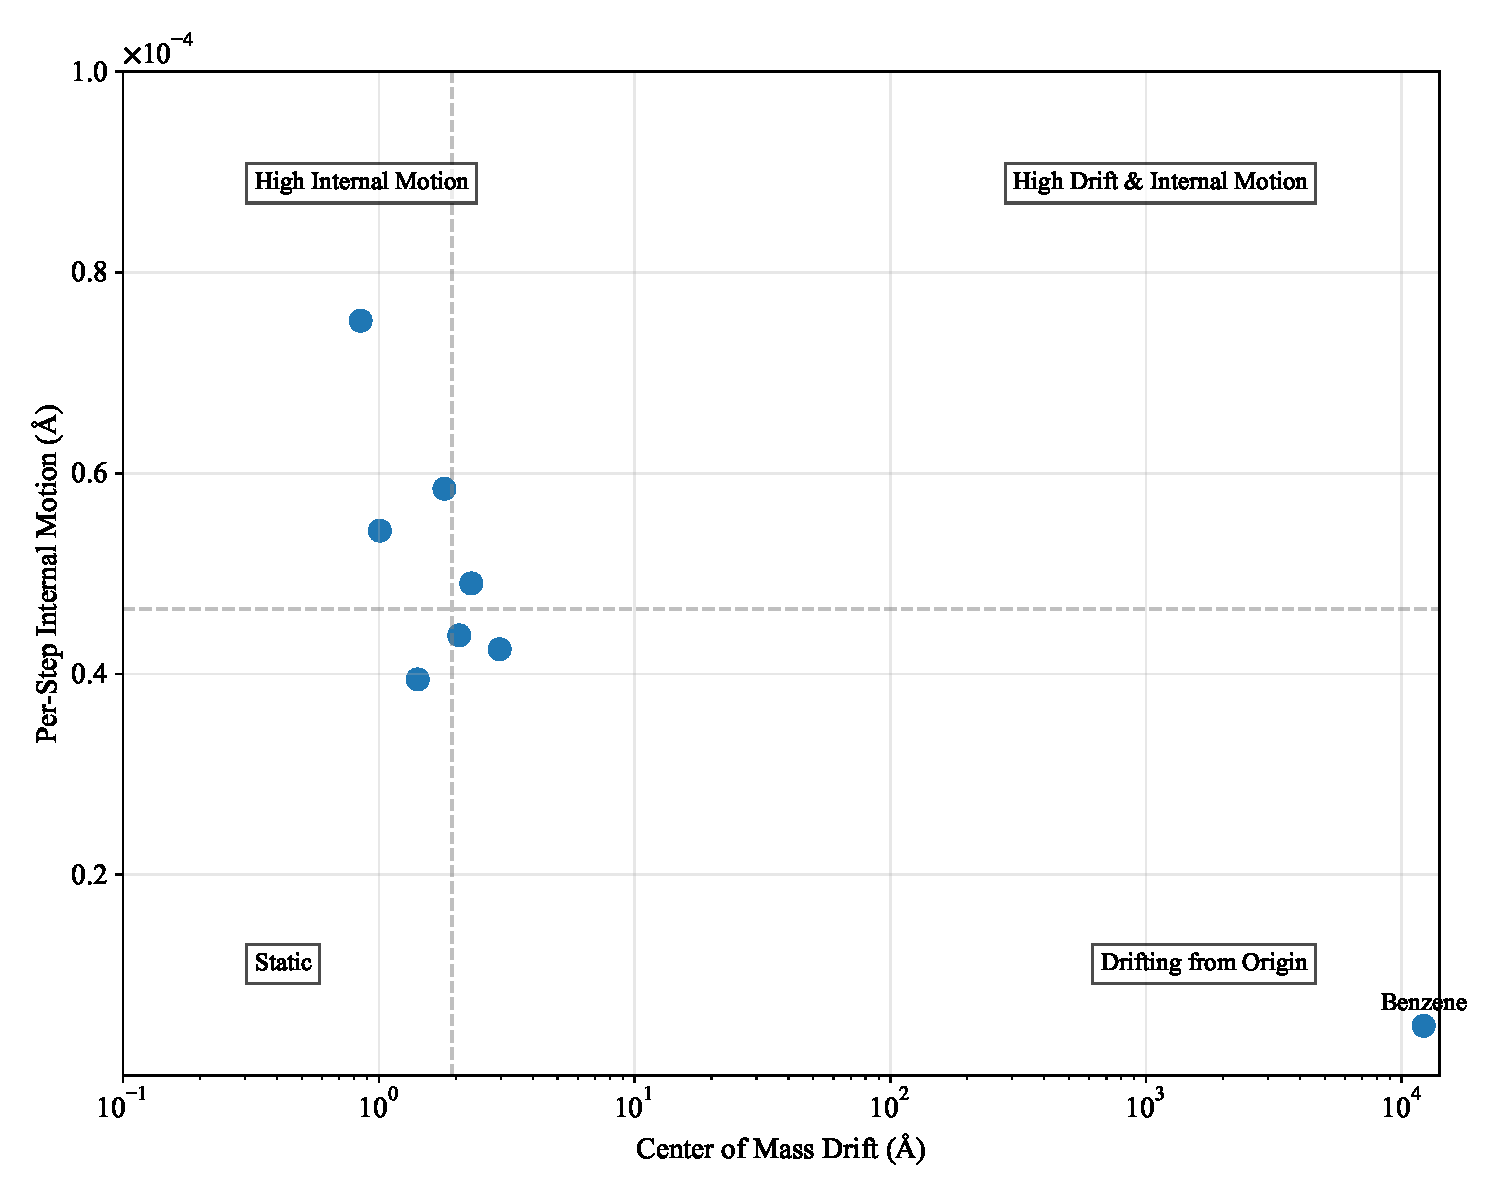
\includegraphics[width=\linewidth]{Figures/dataset/md17_molecule_behavior_comparison.pdf}
        \caption{MD17 molecules are largely consistent, save for benzene, which shows substantial drift.}
        \label{fig:MD17_numerical_quality}
    \end{subfigure}
    \hspace{0.04\textwidth}
    \begin{subfigure}{0.48\textwidth}
        \centering
        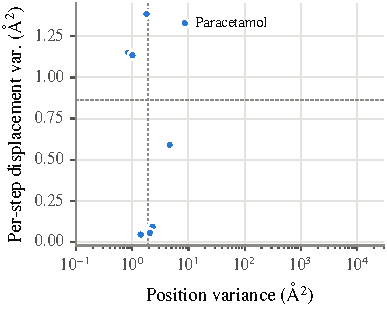
\includegraphics[width=\linewidth]{Figures/dataset/rmd17_molecule_behavior_comparison.pdf}
        \caption{RMD17 molecules exhibit improved numerical stability, supporting their use in future benchmarks.}
        \label{fig:RMD17_numerical_quality}
    \end{subfigure}
        \begin{subfigure}{0.9\textwidth}
        \centering
        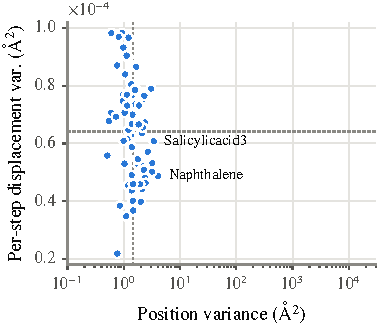
\includegraphics[width=\linewidth]{Figures/dataset/tg80_molecule_behavior_comparison.pdf}
        \caption{TG80 dataset exhibits the lowest centre-of-mass drift among the evaluated MD datasets.}
        \label{fig:TG80_numerical_quality}
    \end{subfigure}
    \caption{Comparison of numerical stability across MD17, RMD17, and TG80 datasets. Dashed lines denote the mean centre-of-mass drift and per-step motion; datapoints exceeding two standard deviations are annotated.}
    \label{fig:numerical_stability}
\end{figure}

\newpage

\subsubsection{Trajectory Samples}
\begin{figure}[H]
    \centering
    \begin{subfigure}{0.48\linewidth}
        \centering
        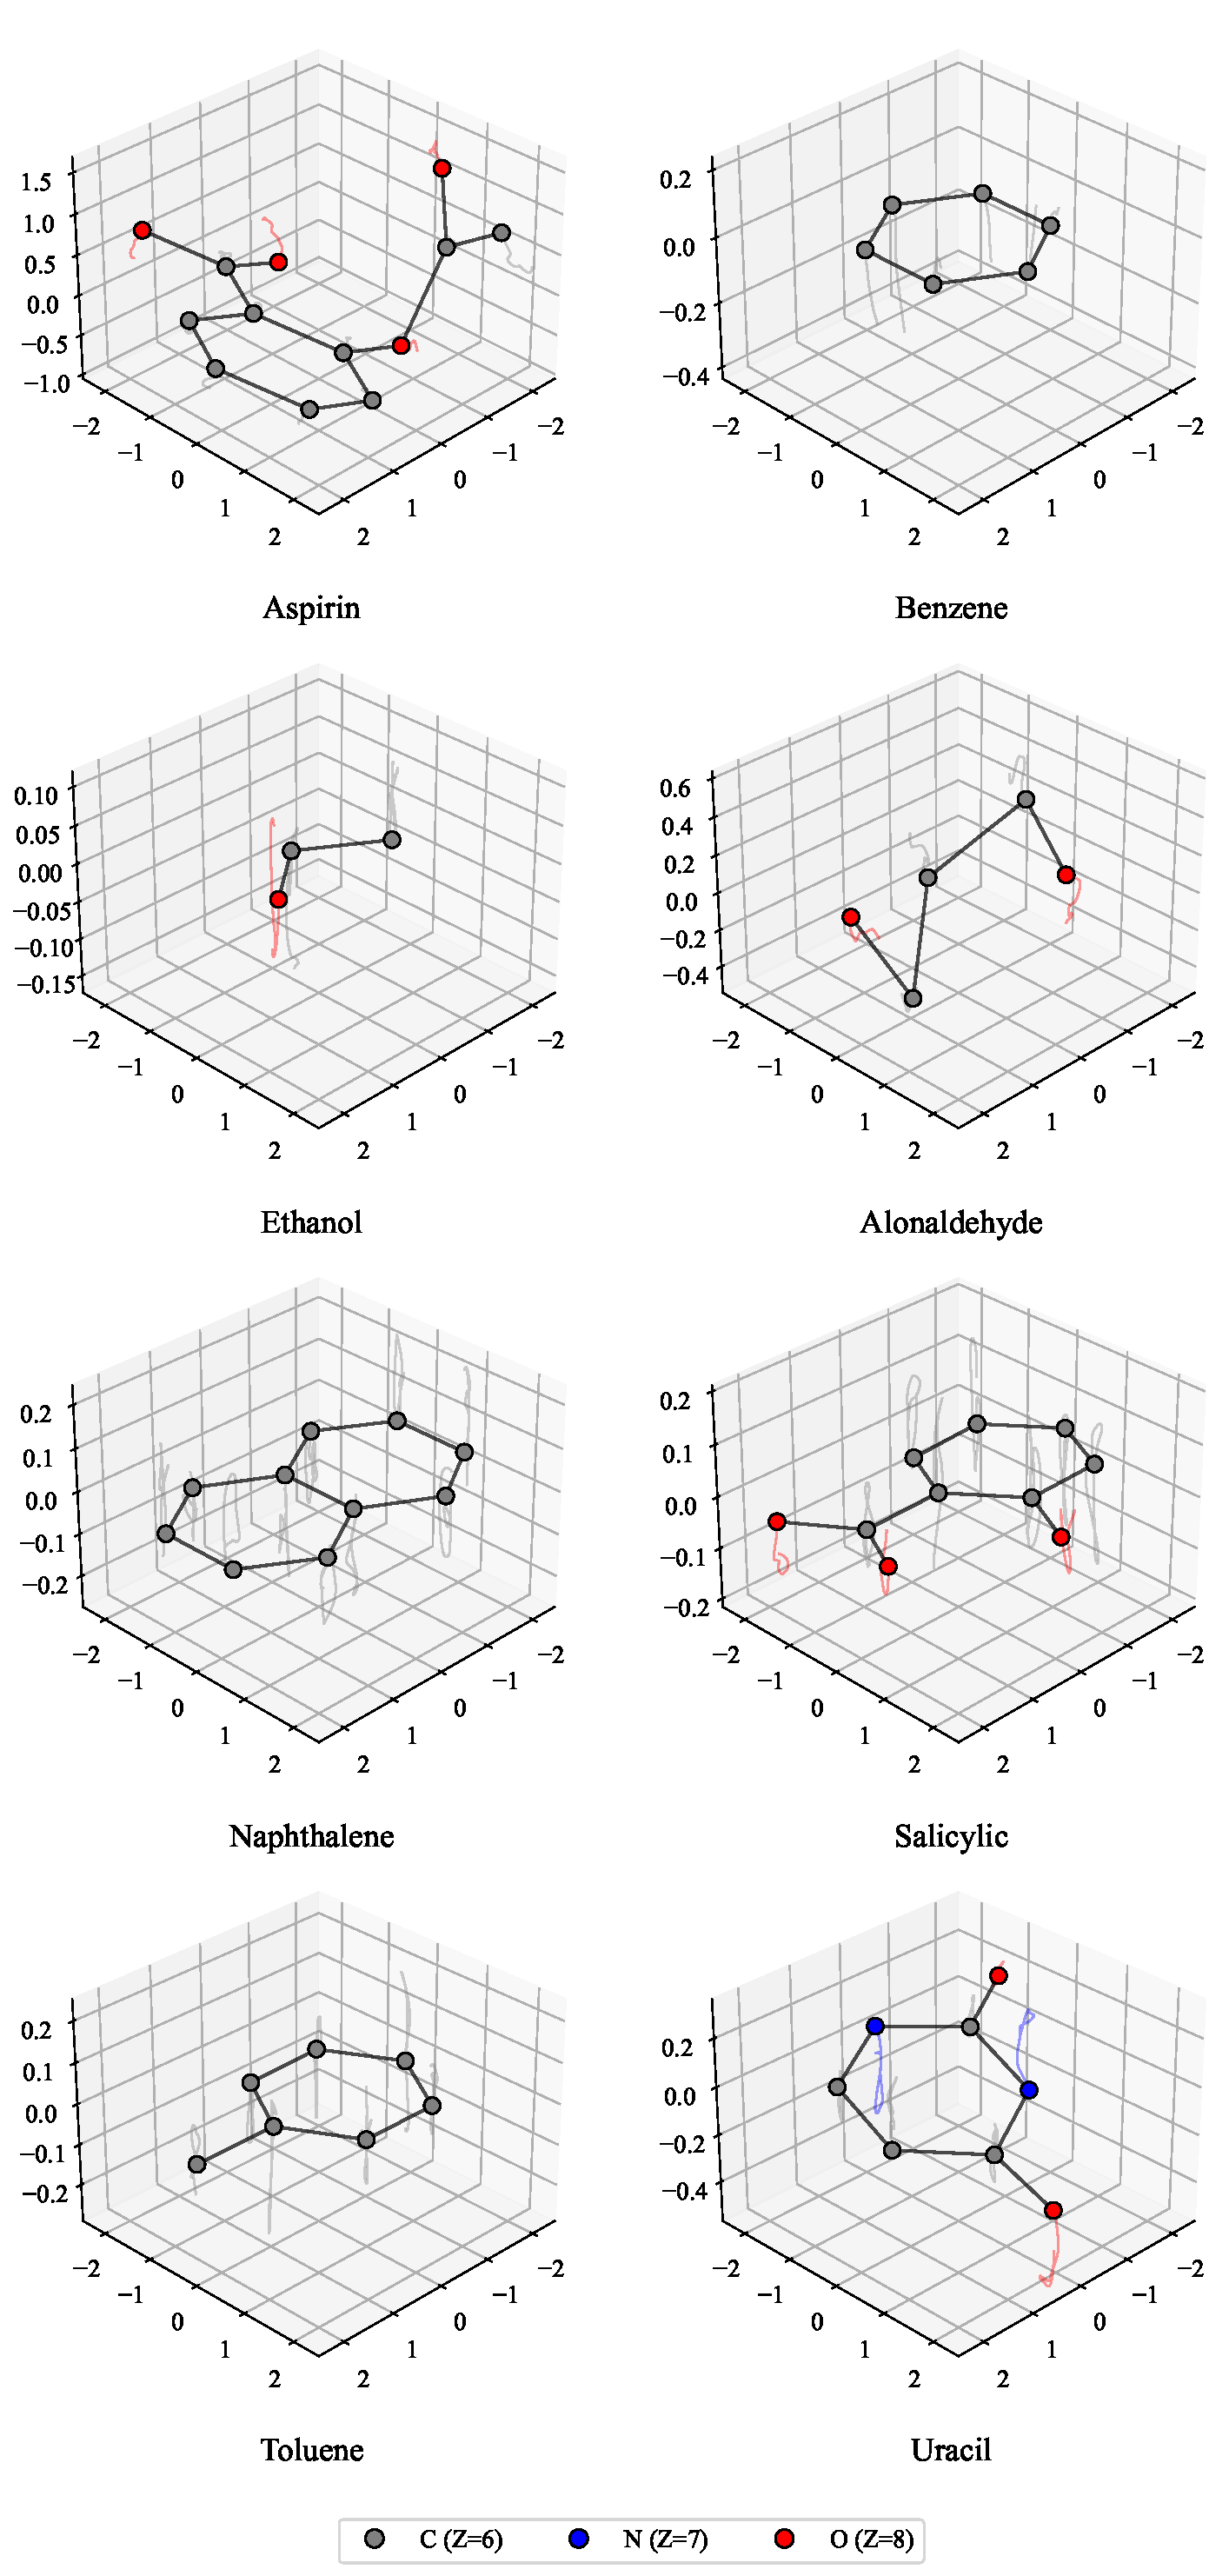
\includegraphics[width=\linewidth]{Figures/dataset/md17_combined_trajectories.pdf}
        \caption{MD17 trajectories}
        \label{fig:MD17_trajectories}
    \end{subfigure}
    \hfill
    \begin{subfigure}{0.48\linewidth}
        \centering
        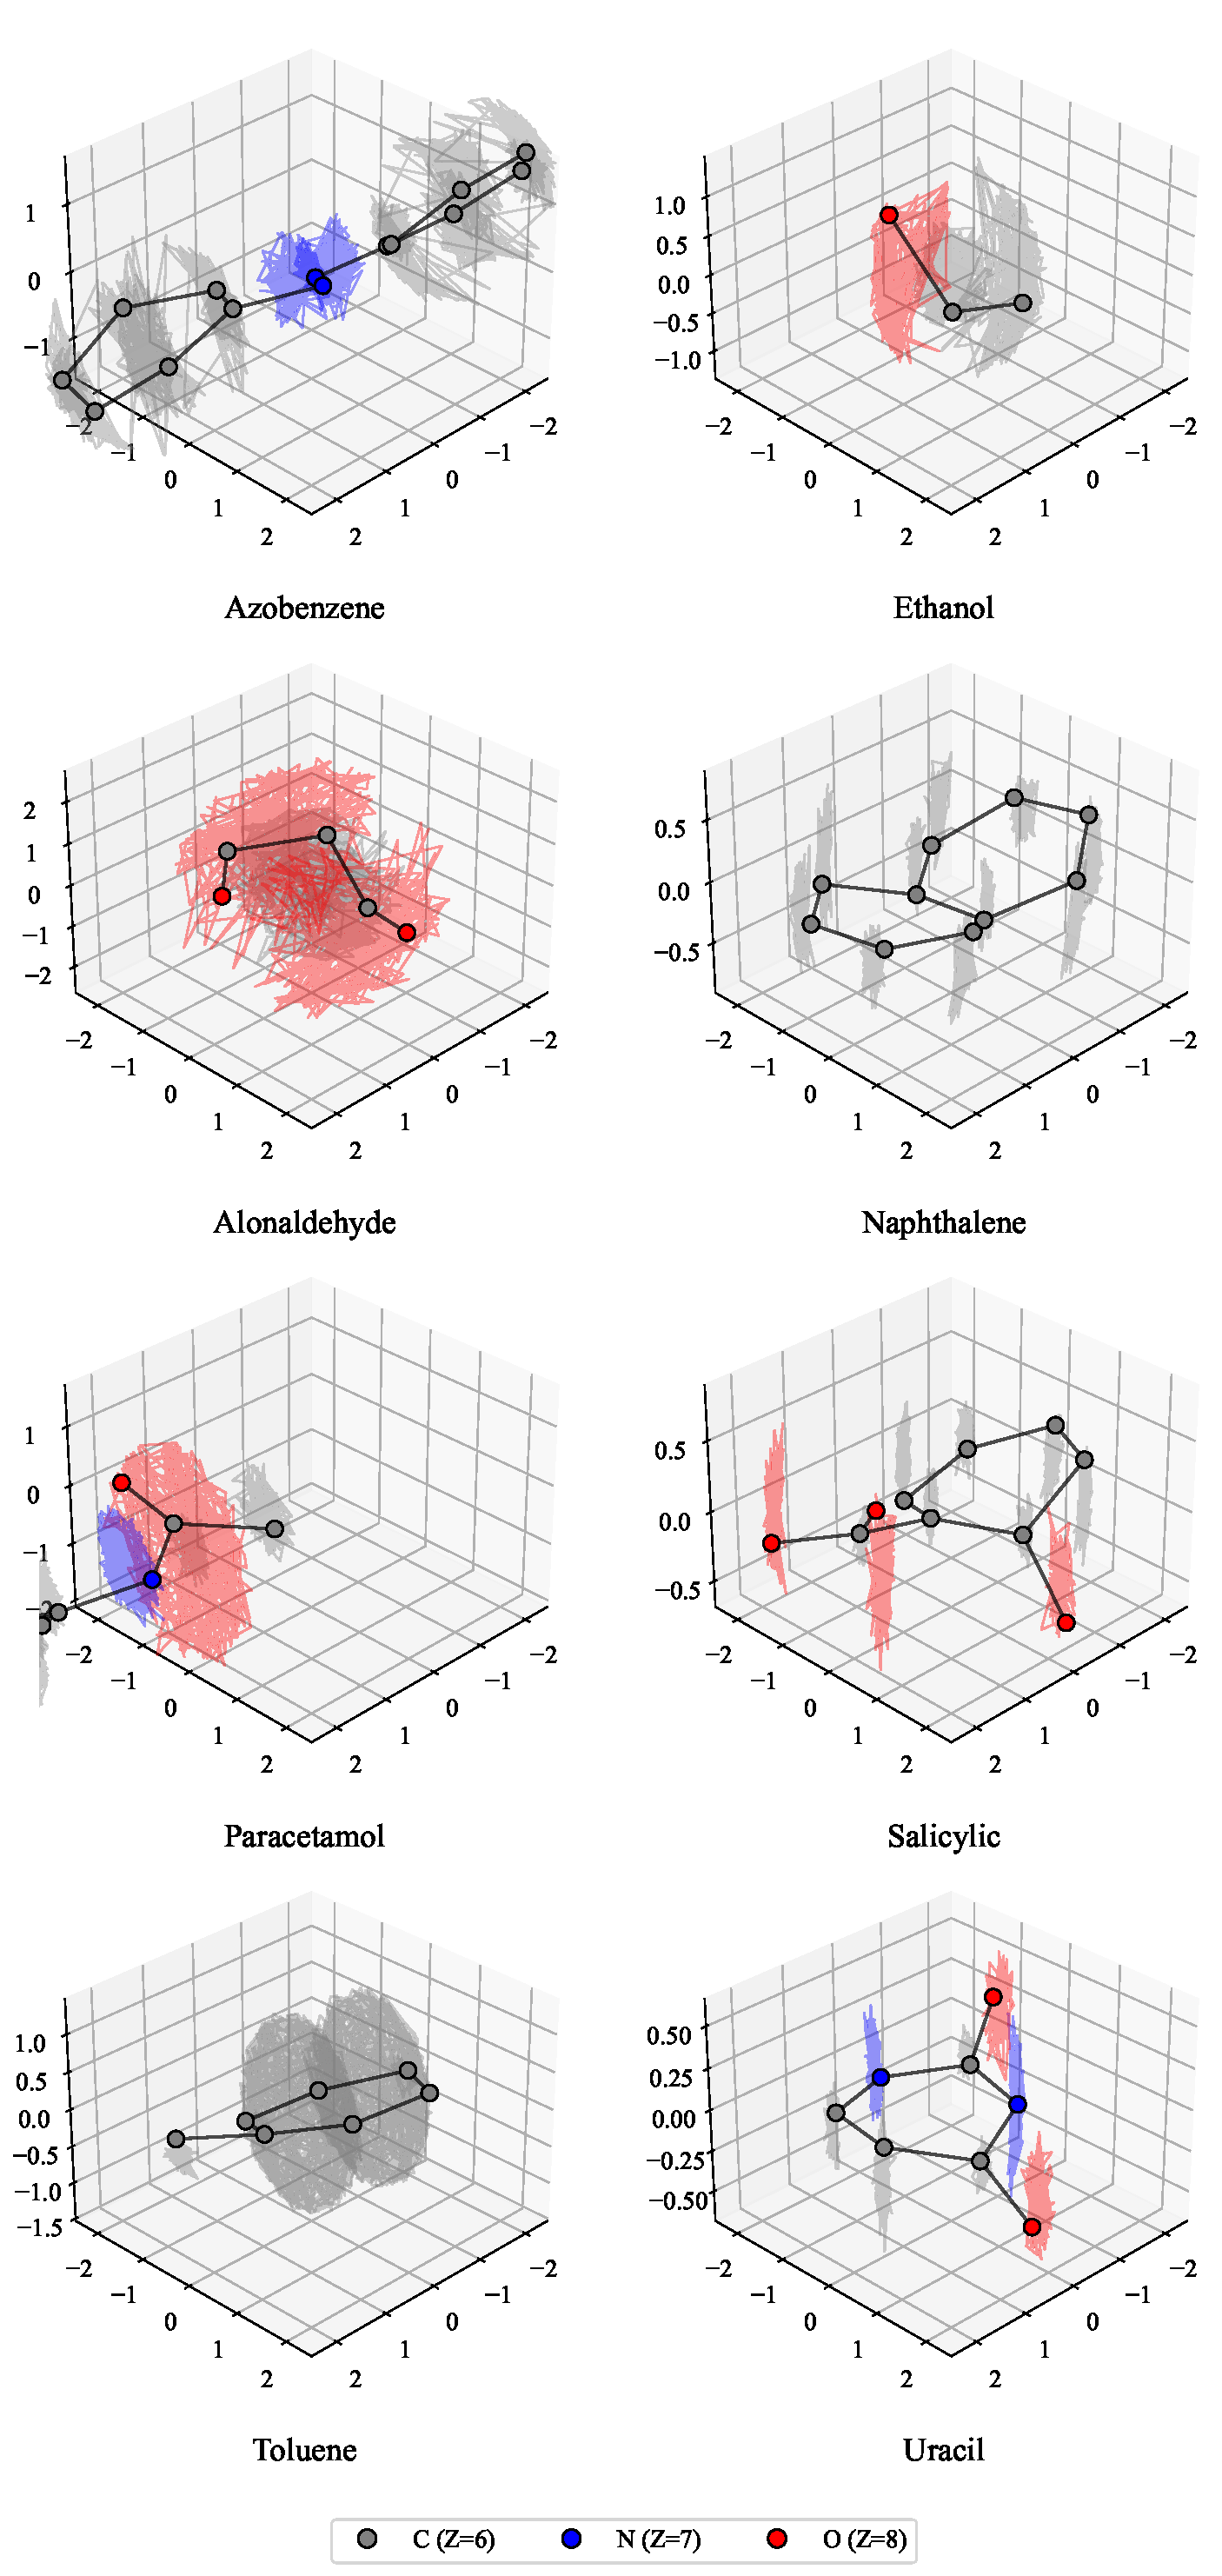
\includegraphics[width=\linewidth]{Figures/dataset/rmd17_combined_trajectories.pdf}
        \caption{RMD17 trajectories}
        \label{fig:RMD17_trajectories}
    \end{subfigure}
    \caption{3000 steps \gls{md} trajectories from the MD17 and RMD17 datasets.}
    \label{fig:trajectories}
\end{figure}

\begin{figure}[H]
    \centering
    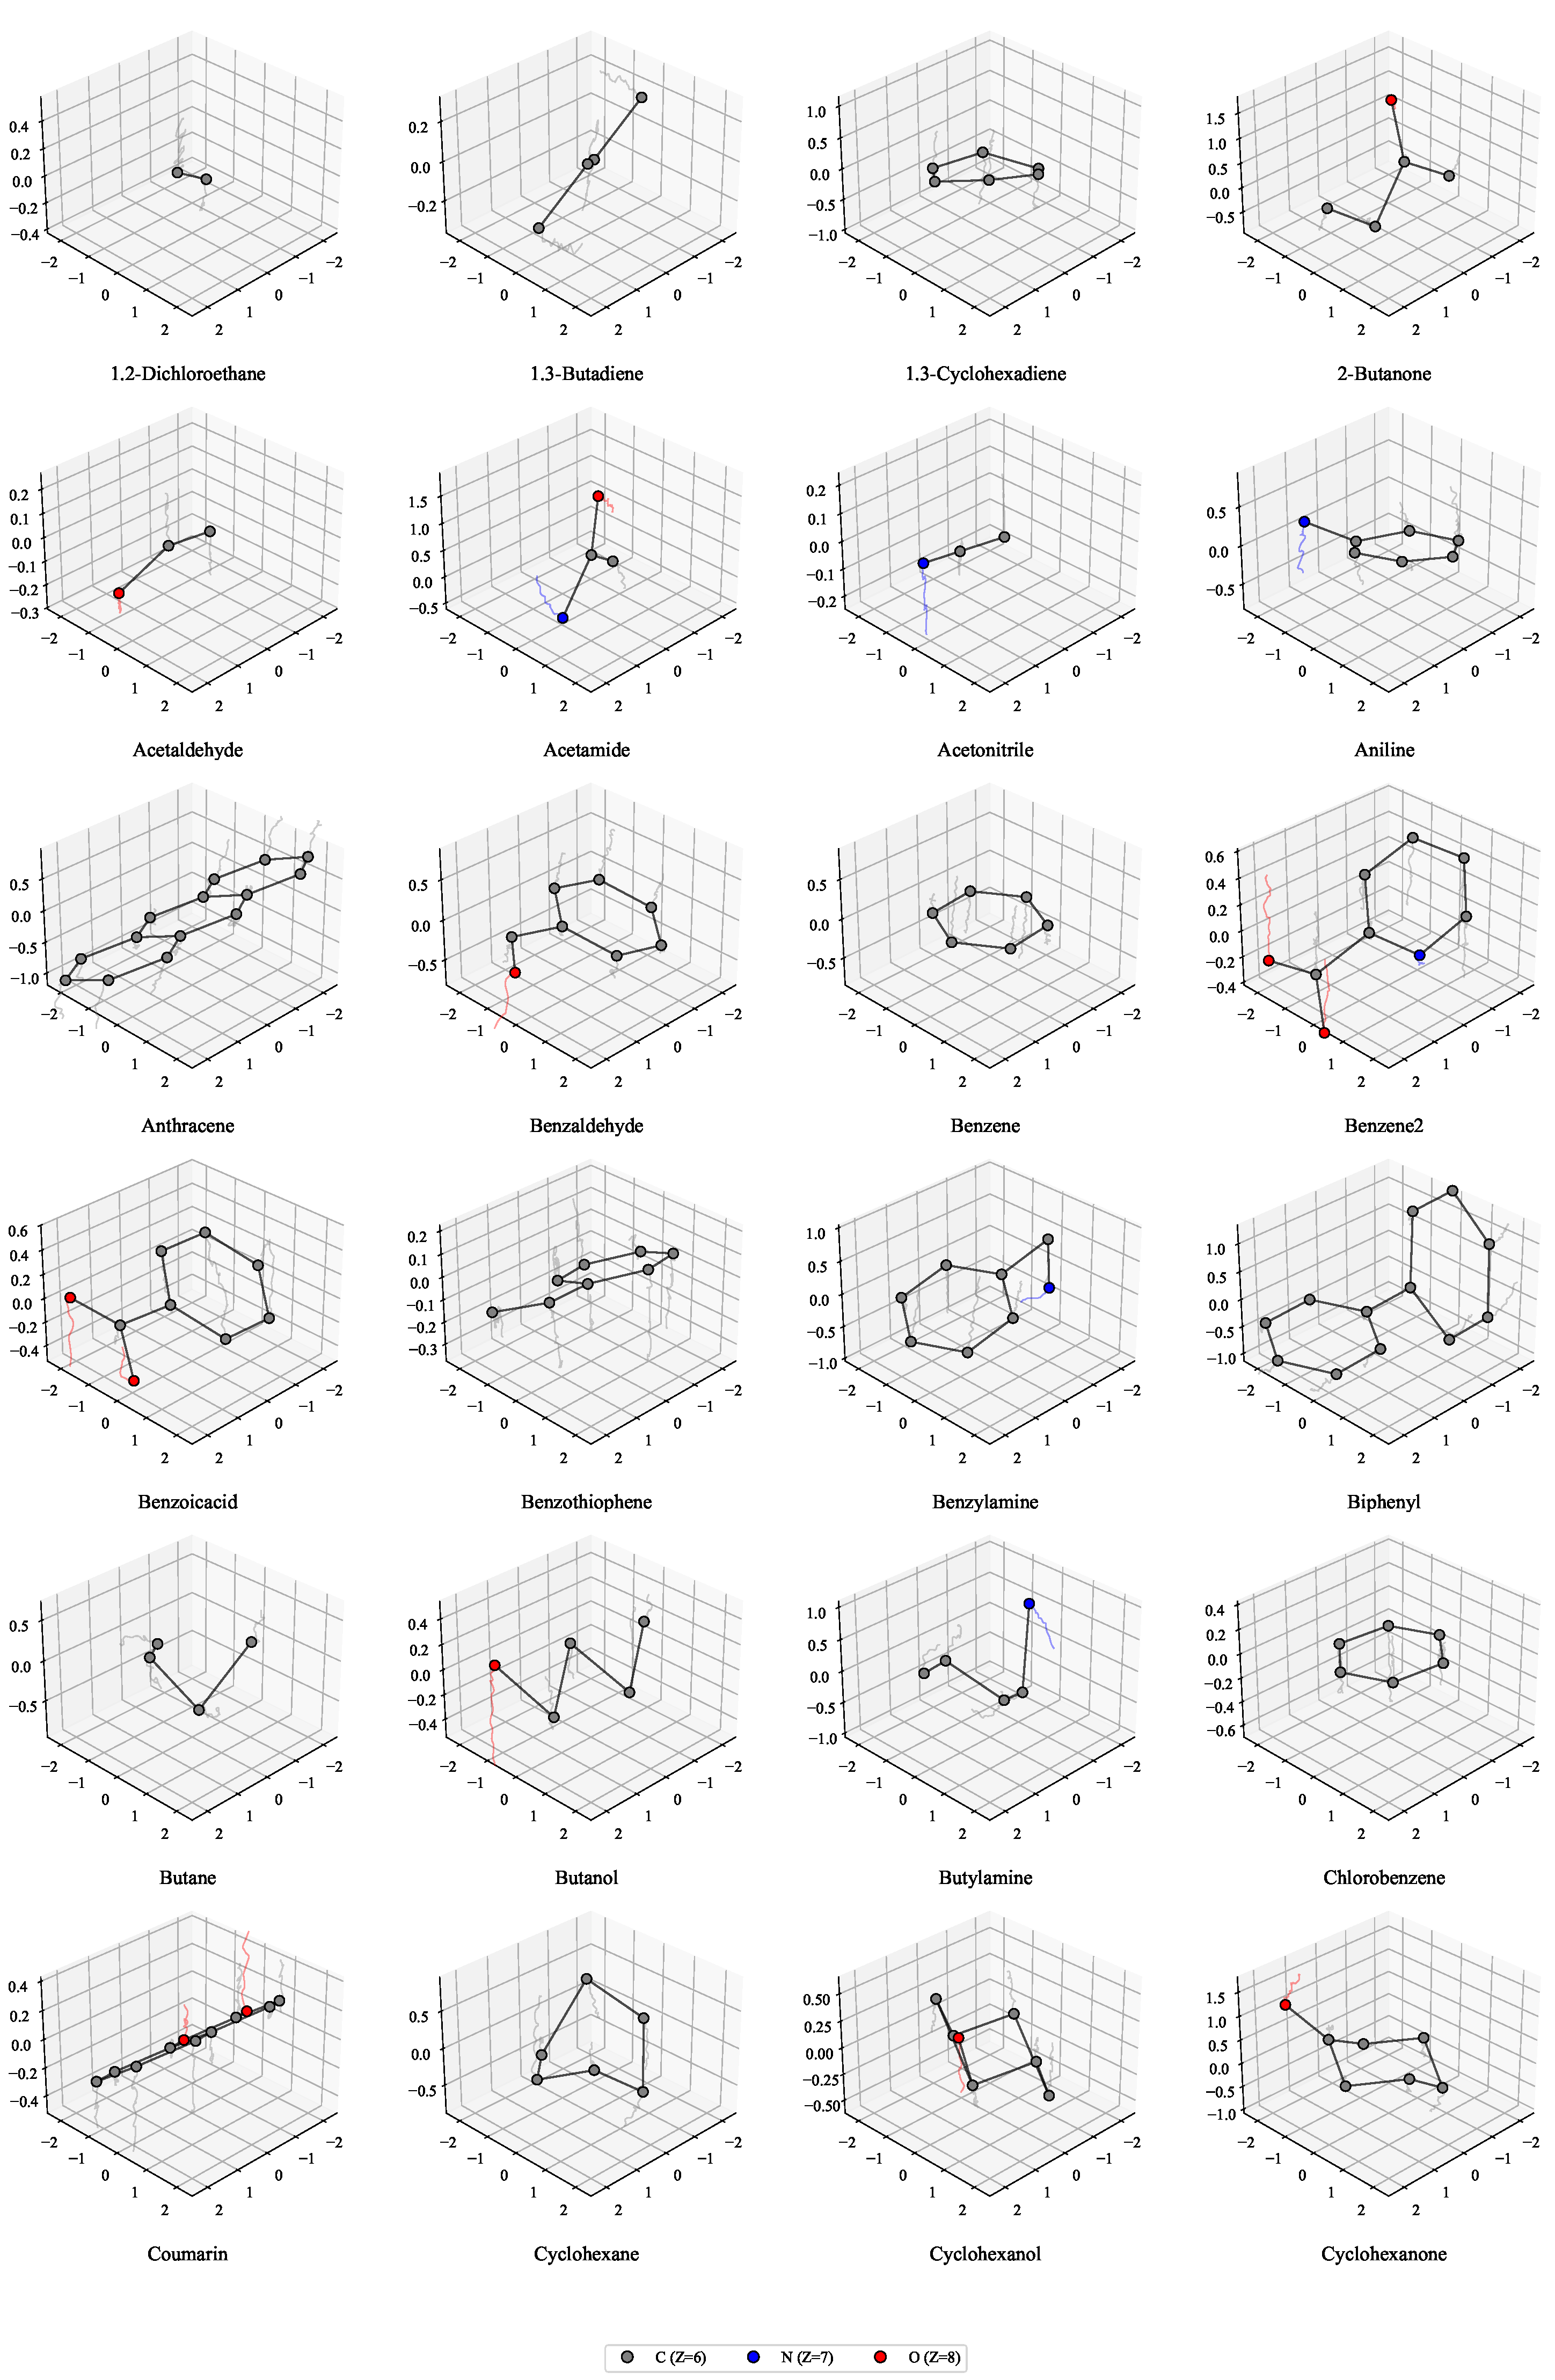
\includegraphics[width=\linewidth]{Figures/dataset/tg80_combined_trajectories_1.pdf}
    \label{fig:TG80_trajectories_1}
\end{figure}
\begin{figure}[H]
    \centering
    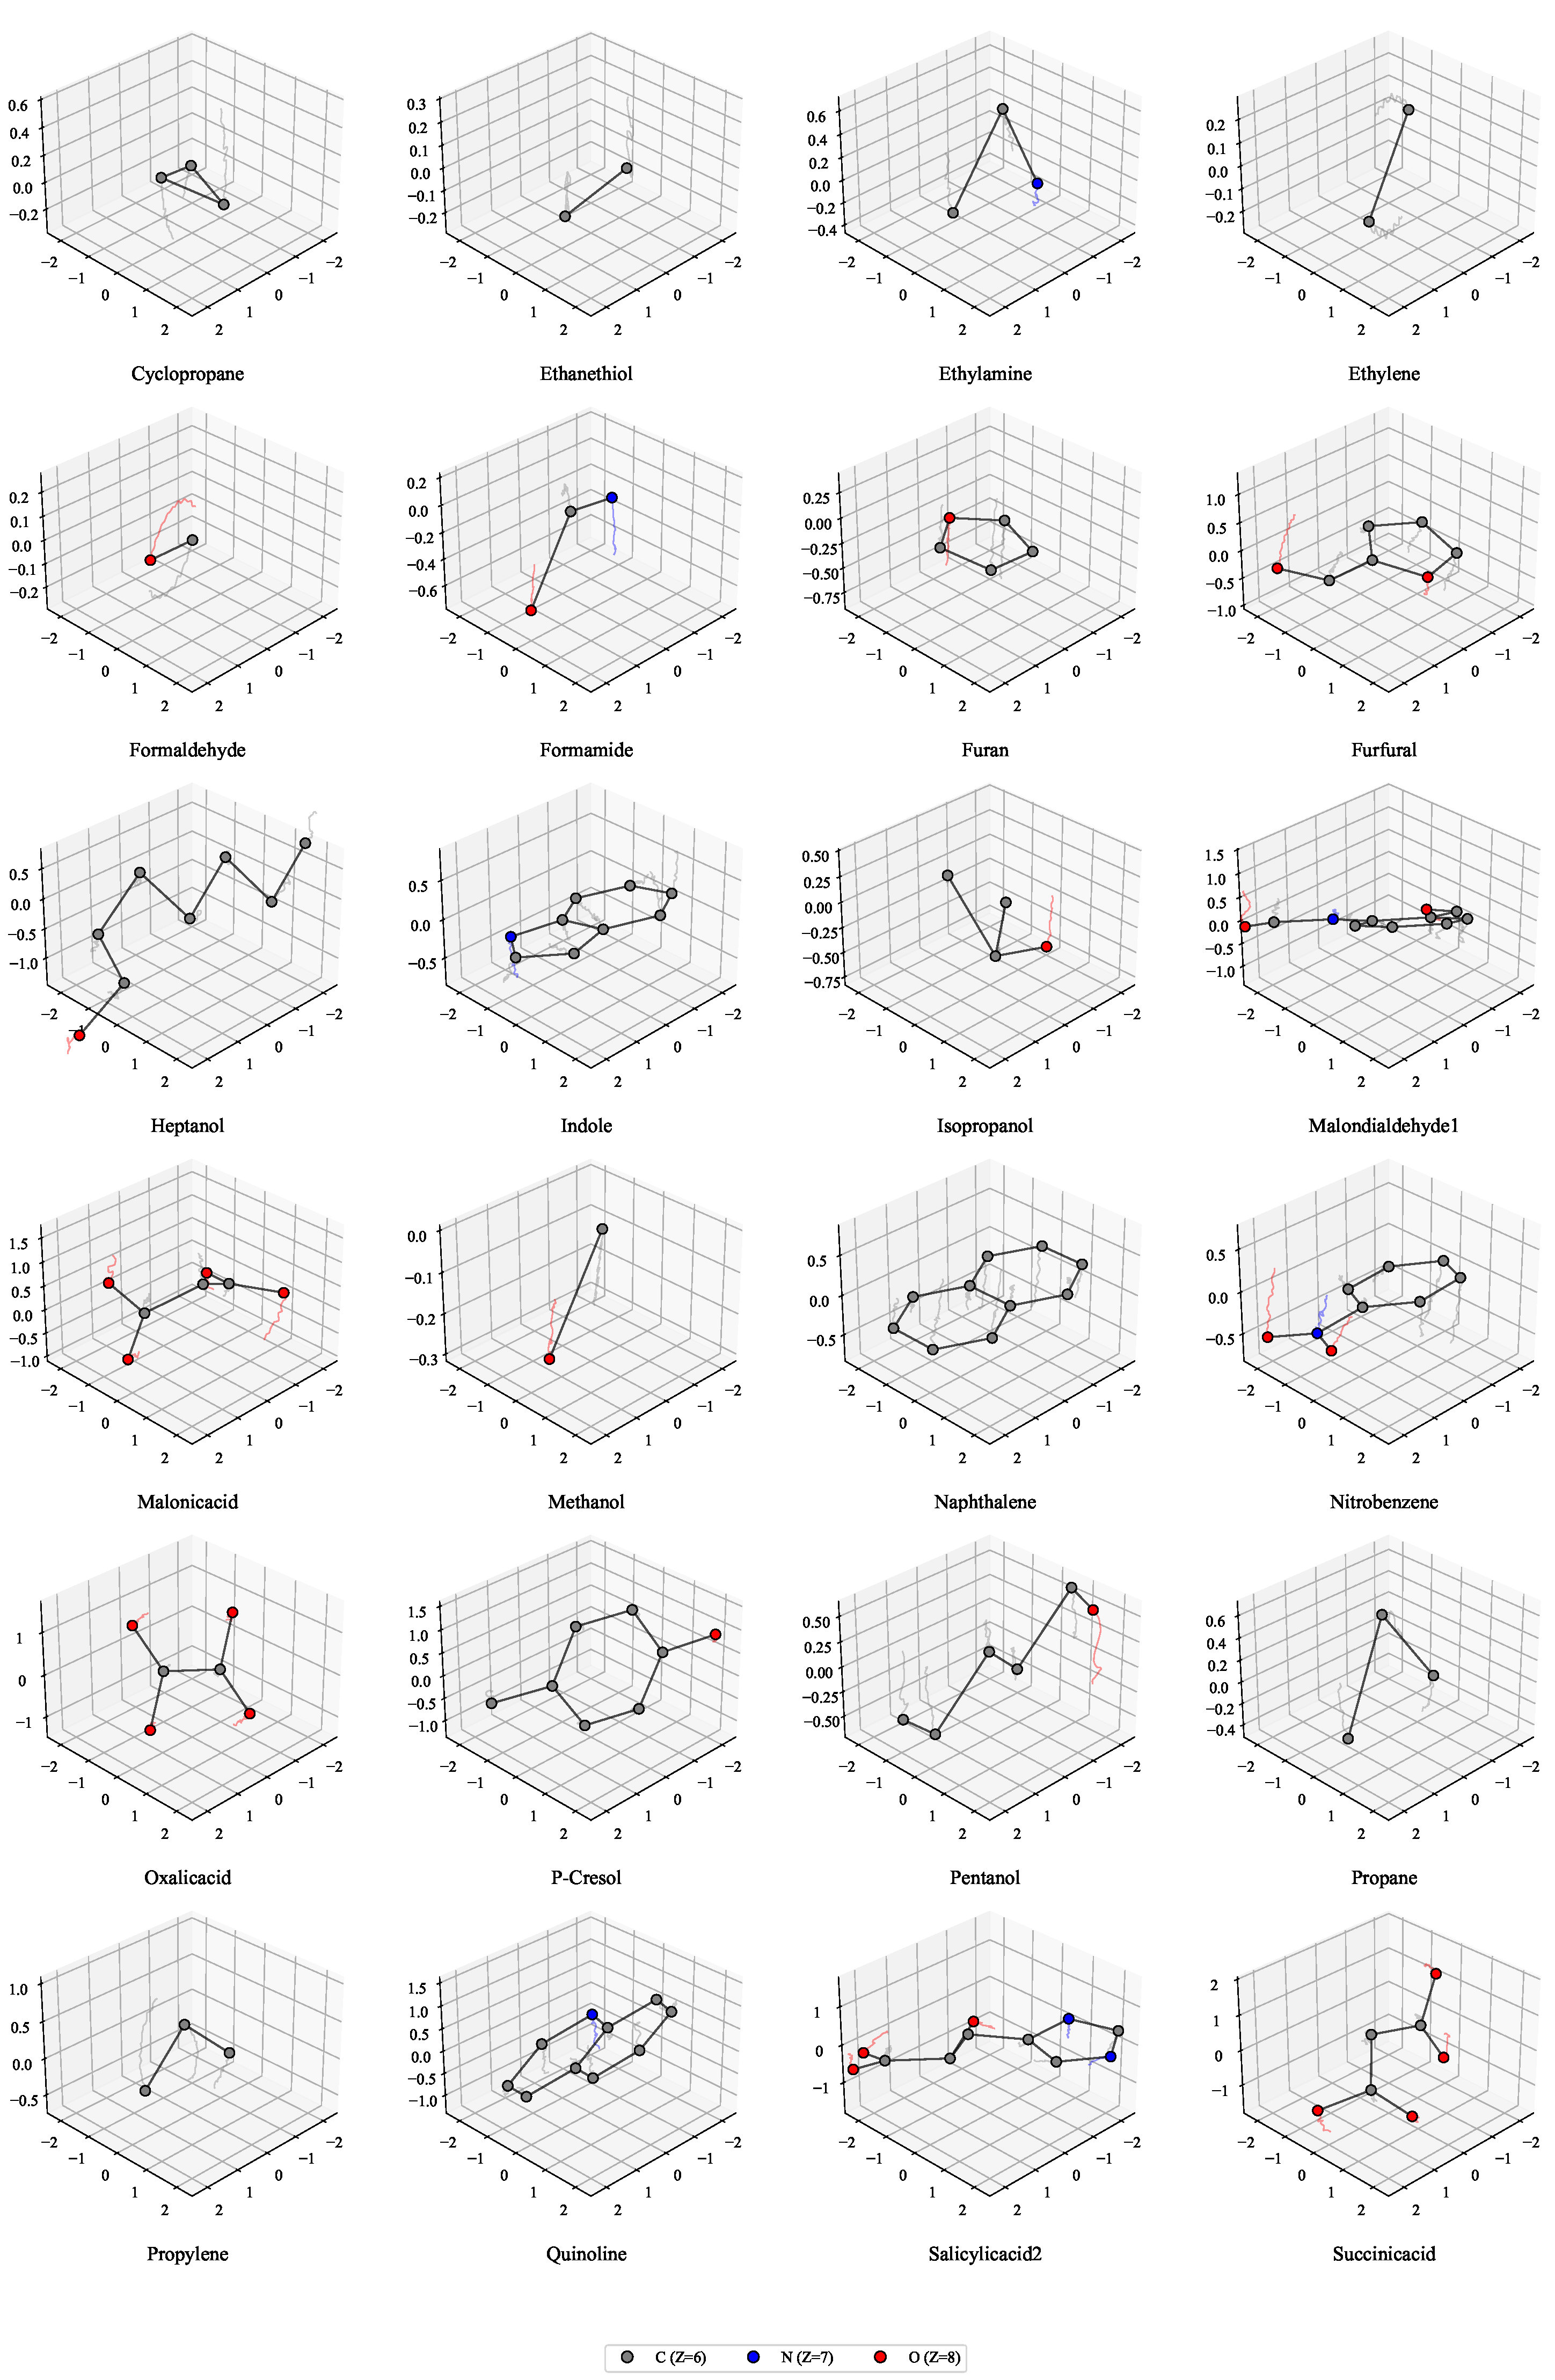
\includegraphics[width=\linewidth]{Figures/dataset/tg80_combined_trajectories_2.pdf}
    \label{fig:TG80_trajectories_2}
\end{figure}
\begin{figure}[H]
    \centering
    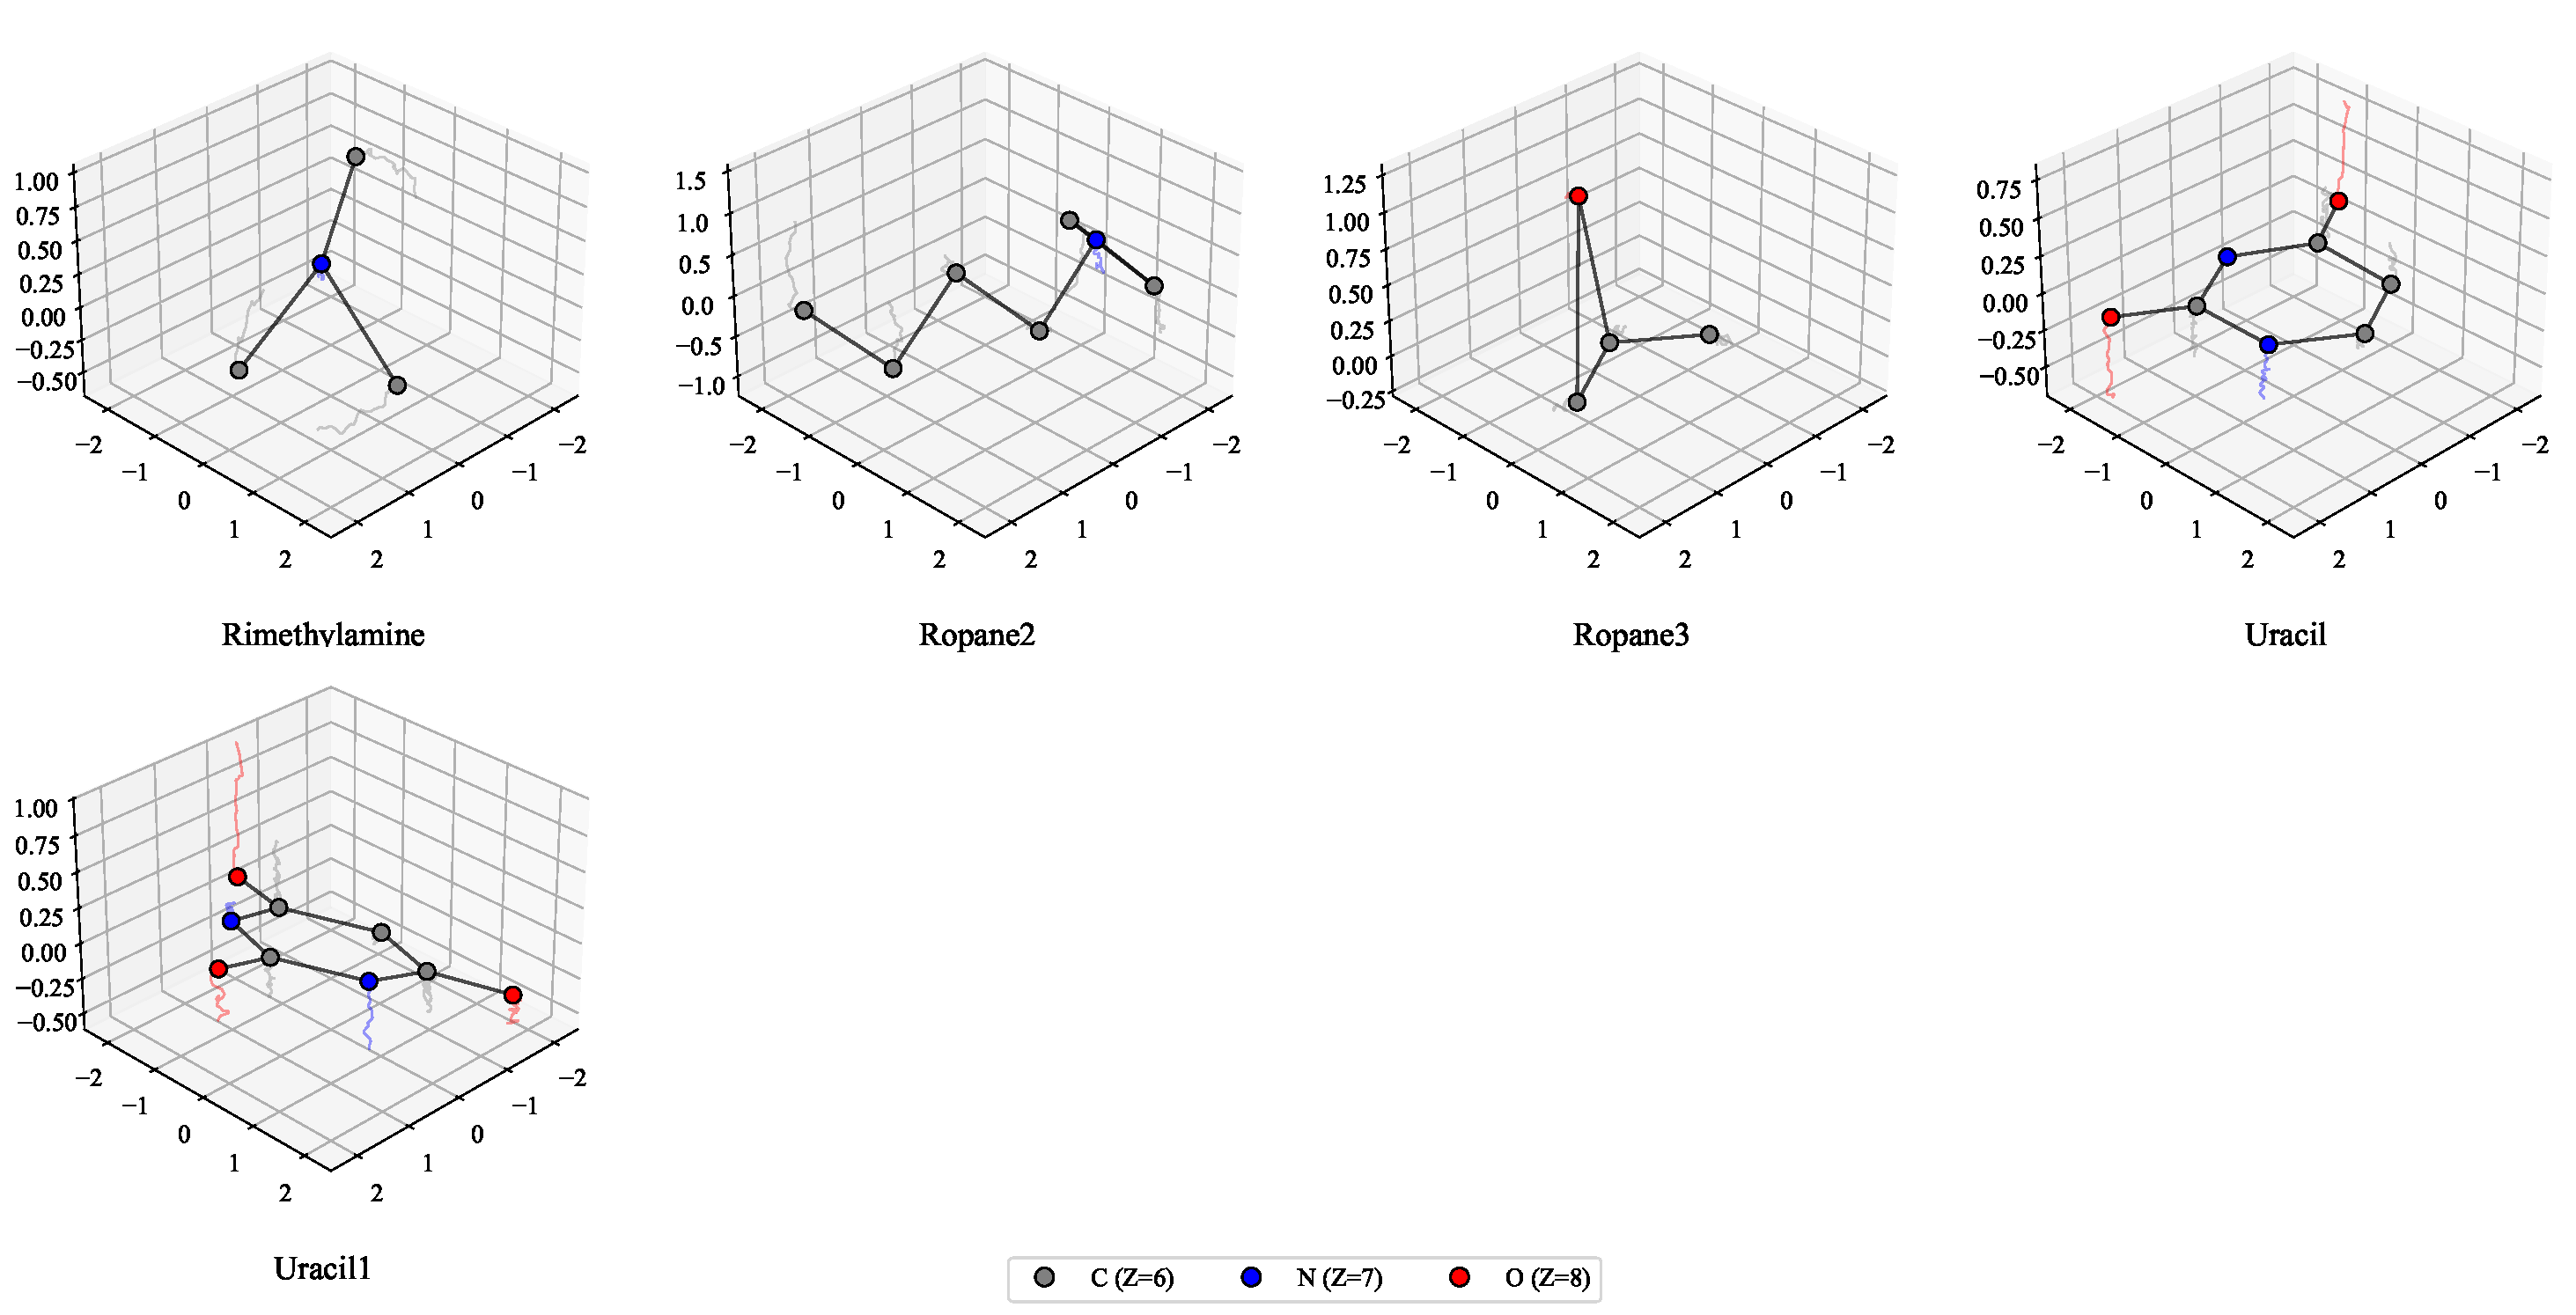
\includegraphics[width=\linewidth]{Figures/dataset/tg80_combined_trajectories_3.pdf}
    \label{fig:TG80_trajectories_3}
    \caption{3000 steps \gls{md} trajectories from the TG80 dataset. Molecules derived from our dataset expansion algorithm are named according to the seed molecule they were related to and their order of selection.}
\end{figure}

\section{Architectural Details}
\subsection{Value-residual Learning}
\label{sec:value_residuals}
We employ value-residual learning, wherein we give every transformer block access to the output of the first block via a residual connection \cite{zhou_value_2024}. This is thought to promote stable training and efficient information flow. Inspired by \cite{jordan_nanogpt_2024}, we add a learned coefficient to weight this residual. Here, \(v\) denotes the current block's value output, and \(v_1\) represents the initial block's value. A learnable parameter \(\alpha\) is passed through a sigmoid to obtain the weighting coefficient:
\begin{equation}
    \lambda = \sigma(\alpha).
\end{equation}
The combined output is then given by
\begin{equation}
    v = \lambda\,v + (1 - \lambda)\,v_1.
\end{equation}
In practice, we lock the first block's \(\lambda\) value to \(0.5\). We report the learned \(\lambda\) values in \cref{fig:lambda_values}.

\begin{figure}[H]
    \begin{subfigure}{0.48\textwidth}
        \centering
        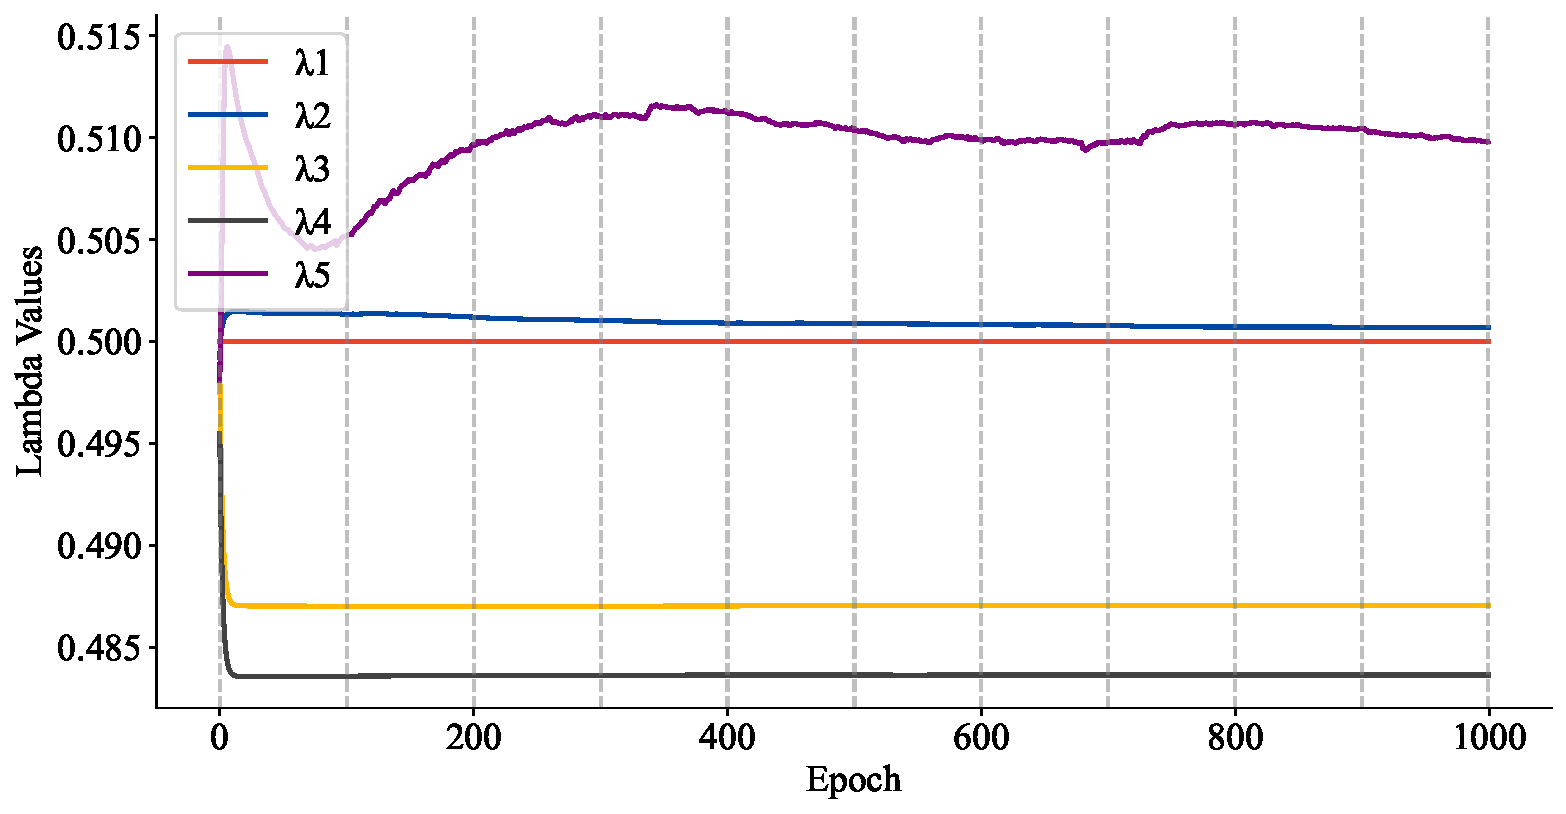
\includegraphics[width=\textwidth]{Figures/lambda_residuals/lambda_values_aspirin.pdf}
        \caption{Aspirin}
    \end{subfigure}
    \hfill
    \begin{subfigure}{0.48\textwidth}
        \centering
        \includegraphics[width=\textwidth]{Figures/lambda_residuals/lambda_values_ethanol.pdf}
        \caption{Ethanol}
    \end{subfigure}
    \begin{subfigure}{0.48\textwidth}
        \centering
        \includegraphics[width=\textwidth]{Figures/lambda_residuals/lambda_values_napthalene.pdf}
        \caption{Napthalene}
    \end{subfigure}
    \hfill
    \begin{subfigure}{0.48\textwidth}
        \centering
        \includegraphics[width=\textwidth]{Figures/lambda_residuals/lambda_values_toluene.pdf}
        \caption{Toluene}
    \end{subfigure}
    
    \caption{Learned \(\lambda\) values for each \gls{atoms} transformer block on four MD17 molecules.}
    \label{fig:lambda_values}
\end{figure}

\subsection{Delta-prediction}
\label{sec:delta_prediction}
When \(\Delta\)-prediction is enabled, as in \cref{fig:MD17_ablation}, we incorporate the initial positions \(\mathbf{x}\) as a residual term, reformulating the model as an operator that learns a displacement field rather than predicting absolute positions. We express this as:
\begin{equation}
    \mathbf{x}^\dagger = \operatorname{Project}(\mathbf{x}_{\text{out}}) + \mathbf{x}.
\end{equation}


In practice, this strategy diminishes performance on all molecules except Benzene. We hypothesize that due to massive positional drift, the network learns to minimize its output and allow the residual to dominate. To test this, we check the model's output norm...

\subsection{Multi-head Output}
\label{sec:multi_head_output}
In the multitask case, we utilize a mixture-of-experts-like system to dynamically weight the contribution of multiple output heads based on global molecular context. In this case, each head is a \(\operatorname{Project}\) \gls{mlp} identical to that described in \cref{sec:project}.

Given a set of phase space vectors \(\{ \mathbf{z}_1, \dots, \mathbf{z}_N \} \subseteq \mathbf{Z} \), we compute the mean pool for the whole molecule:
\begin{equation}
    \bar{\mathbf{z}} = \frac{1}{N} \sum\limits_{\mathbf{z} \in \mathbf{Z}} \mathbf{z}.
\end{equation}
We pass this mean pooled representation through a gating network \(\operatorname{ProjectGate} \colon \mathbb{R}^d \to \mathbb{R}^{\text{n\_proj}}\) where \(\text{n\_proj}\) is the number of \(\operatorname{Project}\) heads. A softmax then generates the head weights:
\begin{equation}
    \mathbf{w} = \operatorname{softmax}(\operatorname{HeadGate}(\bar{\mathbf{z}})),
\end{equation}

This then weights the contribution of each \(\operatorname{Project}\) head to the final output:

\begin{align}
    \mathbf{x}_i^\dagger& = \operatorname{Project}_i(\mathbf{x}_\text{out})
    \\
    \mathbf{x}^\dagger &= \sum\limits_{i=1}^{\text{n\_proj}} w_i \cdot \mathbf{x}_i^\dagger
\end{align}

In the single-task learning case, the update remains exactly as described in \cref{sec:project}.

\section{Further Experiments}
\paragraph{Revised MD17 Dataset}
Using the same dataset parameters as for MD17, we find the performance of \gls{atoms} remains excellent on the denoised revised MD17 (RMD17) dataset, with the most substantial improvement seen on naphtalene \cite{christensen_revised_2020}. Performance is generally more consistent, with fewer major regressions vs \gls{egno}.

\begin{table}[H]
    \centering
    \caption{MSE (\(\times 10^{-2}\)) on RMD17. Upper part: S2S \gls{mse}. Lower part: S2T \gls{mse}}
    \label{tab:rmd17_results}
    \resizebox{\linewidth}{!}{
    \begin{tabular}{lccccccccc}
        \toprule
        & Azobenzene & Ethanol & Malonaldehyde & Naphthalene & Paracetamol & Salicylic & Toluene & Uracil & Mean \% \\
        \midrule
        EGNO & \(10.82{\scriptstyle \pm0.05}\) & \(28.27{\scriptstyle \pm0.16}\) & \(49.25{\scriptstyle \pm0.10}\) & \(1.85{\scriptstyle \pm0.01}\) & \(28.90{\scriptstyle \pm0.20}\) & \(1.26{\scriptstyle \pm0.01}\) & \(28.44{\scriptstyle \pm0.18}\) & \(0.98{\scriptstyle \pm0.01}\) \\
        \gls{atoms} & \(\mathbf{8.36}{\scriptstyle \pm0.01}\) & \(\mathbf{23.81}{\scriptstyle \pm1.29}\) & \(\mathbf{39.87}{\scriptstyle \pm0.53}\) & \(\mathbf{1.42}{\scriptstyle \pm0.01}\) & \(\mathbf{28.74}{\scriptstyle \pm0.33}\) & \(\mathbf{1.09}{\scriptstyle \pm0.01}\) & \(28.48{\scriptstyle \pm0.02}\) & \(\mathbf{0.89}{\scriptstyle \pm0.01}\) \\
        \midrule
        \rowcolor{gray!20} Improvement (\%) & \(22.74\%\) & \(15.78\%\) & \(19.05\%\) & \(23.24\%\) & \(0.55\%\) & \(13.49\%\) & \(-0.14\%\) & \(9.18\%\) & \(\mathbf{12.99\%}\) \\
        
        \midrule
        EGNO & \(10.75{\scriptstyle \pm0.05}\) & \(28.19{\scriptstyle \pm0.16}\) & \(48.78{\scriptstyle \pm0.10}\) & \(1.80{\scriptstyle \pm0.01}\) & \(\mathbf{28.29}{\scriptstyle \pm0.20}\) & \(1.25{\scriptstyle \pm0.01}\) & \(28.37{\scriptstyle \pm0.18}\) & \(0.98{\scriptstyle \pm0.01}\) \\
        \gls{atoms} & \(\mathbf{8.61}{\scriptstyle \pm0.01}\) & \(\mathbf{23.48}{\scriptstyle \pm 
        0.14}\) & \(\mathbf{40.36}{\scriptstyle \pm0.33}\) & \(\mathbf{1.41}{\scriptstyle \pm0.01}\) & \(28.79{\scriptstyle \pm0.33}\) & \(\mathbf{1.08}{\scriptstyle \pm0.01}\) & \(28.45{\scriptstyle \pm0.071}\) & \(\mathbf{0.89}{\scriptstyle \pm0.01}\) \\
        \midrule
        \rowcolor{gray!20} Improvement (\%) & \(19.91\%\) & \(16.71\%\) & \(17.26\%\) & \(21.67\%\) & \(-1.77\%\) & \(13.60\%\) & \(-0.28\%\) & \(9.18\%\) & \(\mathbf{12.04\%}\) \\
        \bottomrule
    \end{tabular}
    }
\end{table}

\subsection{Explicit hydrogen representation}
We hypothesized that our model's underperformance relative to \gls{egno} on malonaldehyde was due to the omission of explicit hydrogens, limiting its ability to capture electron delocalization effects involving hydroxyl hydrogens. We tested two explicit hydrogen methods: 
\begin{enumerate}
    \item Including all hydrogens with gradients computed for all atoms during training
    \item Including all hydrogens but computing gradients only for heavy atoms
\end{enumerate}

Contrary to conventional \gls{md} practice, neither method improved heavy-atom test loss.

\begin{table}[H]
    \centering
    \caption{\gls{atoms} S2T MSE loss with implicit hydrogens and two explicit hydrogen approaches.}
    \label{tab:explicit_hydrogens}
    \begin{tabular}{lcc}
        \toprule
        & Aspirin & Malonaldehyde \\
        \midrule
        Implicit hydrogens &  \\
        Explicit hydrogens 1 & \(7.48{\scriptstyle \pm0.11}\) & \(15.15{\scriptstyle \pm0.22}\) \\
        Explicit hydrogens 2 & \(6.96{\scriptstyle \pm0.20}\) & \(13.52{\scriptstyle \pm0.10}\)\\
        \bottomrule
    \end{tabular}
\end{table}

\subsection{Learnable attention denominator}
Following \textcite{jordan_nanogpt_2025} and correspondence with the authors, we experimented with a learnable per-head attention scale and initialized it to the standard \(d_k\). Specific ablation studies on aspirin, ethanol, naphthalene, and toluene failed to improve \gls{mse} significantly. We also found that the change in values over the course of training was minimal, in the order of \(2\%\).

\begin{table}[H]
    \centering
    \caption{MSE (\(\times 10^{-2}\)) with and without learnable attention denominators across four MD17 compounds. Upper part: S2S. Lower part: S2T.}
    \label{tab:att_denom}
    \begin{tabular}{lcccc}
        \toprule
        & Aspirin & Ethanol & Napthalene & Toluene \\
        \midrule
         Standard & \(\mathbf{6.52}{\scriptstyle \pm0.04}\) & \(\mathbf{3.47}{\scriptstyle \pm0.05}\) & \(\mathbf{0.40}{\scriptstyle \pm0.01}\) & \(4.68{\scriptstyle \pm0.17}\) \\
         Learnable denom & \(6.89{\scriptstyle \pm0.21}\) & \(3.65{\scriptstyle \pm0.12}\) & \(0.41{\scriptstyle \pm0.00}\) & \(\mathbf{4.35}{\scriptstyle \pm0.24}\) \\
         \midrule
         Standard & \(\mathbf{5.45}{\scriptstyle \pm0.14}\) & \(\mathbf{2.69}{\scriptstyle \pm0.05}\) & \(\mathbf{0.37}{\scriptstyle \pm0.01}\) & \(2.26{\scriptstyle \pm0.07}\) \\
         Learnable denom & \(5.62{\scriptstyle \pm0.24}\) & \(2.81{\scriptstyle \pm0.09}\) & \(0.38{\scriptstyle \pm0.00}\) & \(\mathbf{2.13}{\scriptstyle \pm0.09}\) \\
        \bottomrule
    \end{tabular}
\end{table}


\begin{figure}[H]
    \begin{subfigure}{0.48\textwidth}
        \centering
        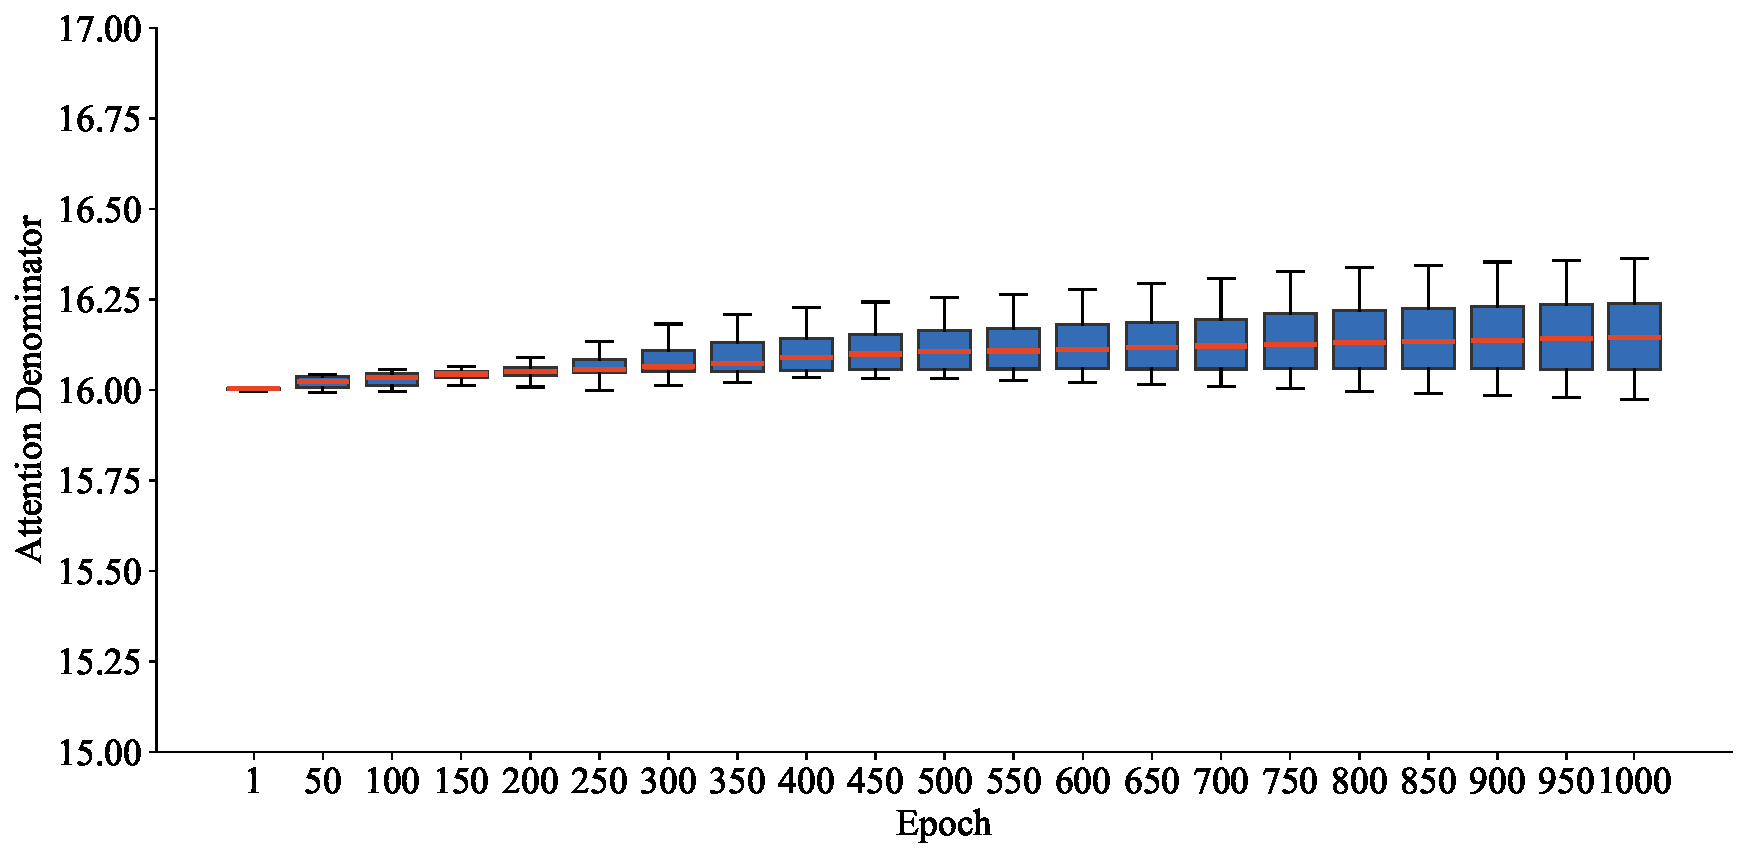
\includegraphics[width=\textwidth]{Figures/attention_denoms/attention_weights_aspirin.pdf}
        \caption{Aspirin}
    \end{subfigure}
    \hfill
    \begin{subfigure}{0.48\textwidth}
        \centering
        \includegraphics[width=\textwidth]{Figures/attention_denoms/attention_weights_ethanol.pdf}
        \caption{Ethanol}
    \end{subfigure}
    \begin{subfigure}{0.48\textwidth}
        \centering
        \includegraphics[width=\textwidth]{Figures/attention_denoms/attention_weights_napthalene.pdf}
        \caption{Napthalene}
    \end{subfigure}
    \hfill
    \begin{subfigure}{0.48\textwidth}
        \centering
        \includegraphics[width=\textwidth]{Figures/attention_denoms/attention_weights_toluene.pdf}
        \caption{Toluene}
    \end{subfigure}
    
    \caption{Learned attention denominators for aspirin of the MD17 dataset on \gls{atoms}. Each box contains 40 denominators (five layers \(\times\) eight heads).}
    \label{fig:attention_denoms}
\end{figure}

\section{Experimental Details}
\subsection{Software and Hardware Details}
All experiments were conducted using Python 3.12, NumPy 2.2.1 \cite{harris_array_2020}, PyTorch 2.5.1 \cite{paszke_pytorch_2019}, e3nn 0.5.6 \cite{geiger_e3nn_2022} and PyTorch Optimizer 3.5.0 \cite{kim_pytorch_optimizer_2021}. We use RDKit 2024.9.6 \cite{greg_landrum_rdkit_2012} and PubChemPy 1.0.4 in the construction of TG80. All training was performed on an NVIDIA Titan V (12 GB) running CUDA 12.4 on Ubuntu 24.04.

\subsection{\gls{atoms} Hyperparameters}
\label{sec:my_hyperparams}
We employ the same dataset splitting and discretization parameters reported in \textcite{xu_equivariant_2024} for the MD17 and \(N\)-body simulation tasks. We set the batch size to \(100\) to ensure complete batches and avoid Torch graph breaks, given our dataset sizes are multiples of \(100\). We reduce the AdamW \(\epsilon\) to \(1\times10^{-10}\) to avoid instability associated with the small gradients produced by zero-initialised weight matrices in early training \cite{jordan_nanogpt_2025}. We present a complete overview of our hyperparameters in \cref{tab:gtno_hparams}.

\begin{table}[h]
    \centering
    \caption{Hyperparameters for \gls{atoms}. MD17 hyperparameters are shared across all molecules unless otherwise noted.}
    \label{tab:gtno_hparams}
    \begin{tabular}{cccc}
        Module & & MD17, RMD17 Value & TG80 Multitask \\
        % Module & & MD17, RMD17 Value & \(N\)-body Value & Multitask \\
        \midrule
        Training & & \\
        & Batch size & \( 100 \) & \( 192 \) \\
        & Epochs & \( 1000 \) & \(250\) \\
        & Max grad norm & \( 1.0 \) & \(1.0\) \\
        & Noise \(\sigma\) & \( 0.1 \) & \(0.1\) \\
        & \(\Delta t\) & \( 3000 \) & \( 10\ 000 \) \\
        & Timesteps \(P\) & \( 8 \) & \( 8 \) \\
        & Train/Val/Test & \( (500,3000,3000) \) & \( (500,3000,3000) \) \\
        \midrule
        Optimiser & & \\
        & Optimiser type & AdamW-AMSGrad\cite{loshchilov_decoupled_2017} & Muon \cite{jordan_muon_2024, kim_pytorch_optimizer_2021}  \\
        & Learning rate & \( 1\times10^{-3} \) & \( 1\times10^{-3} \) \\
        & \(\beta_1, \beta_2\) & \( 0.9, 0.999 \) & N/A \\
        & Weight decay & \( 1\times10^{-5} \) & \( 1\times10^{-5} \) \\
        & \(\epsilon\) & \( 1\times10^{-10} \) & \( 1\times10^{-5} \) \\
        \midrule
        Model & & \\
        & Embedding dim & \( 128 \) & \( 128 \) \\
        & No. layers & \( 5 \) & \( 5 \) \\
        & No. attention heads & \( 8 \) & \( 8 \) \\
        & No. output heads & \(1\) & \(8\) \\
        & Attention dropout & \( 0.2 \) & \( 0.2 \) \\
        & RoPE frequency & \( 1000 \) & \( 1000 \)\\
        & MLP layers & \( 2 \) & \( 2 \) \\
        & MLP activation & SwiGLU & SwiGLU \\
        & MLP dropout & \( 0.0 \) & \( 0.0 \) \\
        & Norm type & RMS norm & RMS norm \\
        & Learnable value residuals & True & True \\
        & Spherical harmonic bias & False & False \\
        \bottomrule
    \end{tabular}
\end{table}
